\documentclass[12pt,a4paper]{article}

\usepackage[margin=1in]{geometry}
\usepackage[T1]{fontenc}
\usepackage{lmodern}
\usepackage{setspace}
\usepackage{hyperref}
\usepackage{enumitem}
\usepackage{microtype}
\usepackage{graphicx}
\usepackage{float}

\hypersetup{
    colorlinks=true,
    linkcolor=black,
    citecolor=black,
    urlcolor=blue,
    pdftitle={Impact of Artificial Intelligence on Students' Studies}
}

\setstretch{1.25}
\setlist[itemize]{leftmargin=1.5em}
\setlist[enumerate]{leftmargin=1.8em}

\title{\textbf{A Case Study on the Impact of Artificial Intelligence on Students' Studies}}

\author{
    Gokulramanan V.\\
    Artificial Intelligence and Data Science,\\
    College of Engineering, Guindy,\\
    Anna University,\\
    Chennai, Tamil Nadu, India\\
    \texttt{gokulramananvec@gmail.com}
}

\date{\today}

\begin{document}

\maketitle
\section{Introduction}

Artificial Intelligence (AI) is becoming increasingly common in education. Students use AI tools to understand difficult concepts, summarize notes, solve problems, and prepare for examinations. These tools can make learning more convenient, but they may also provide inaccurate information or encourage overdependence. This case study explores students' experiences and opinions about the advantages and disadvantages of AI in their studies through a structured questionnaire.

\section{Objectives of the Study}

The main objective of this study is to understand students' experiences and perceptions of AI in education. The specific objectives are:

\begin{enumerate}
    \item To examine students' AI usage habits and the purposes for which they use AI in their studies.
    \item To identify the perceived advantages of AI, including improved understanding, convenience, and time-saving.
    \item To explore concerns related to AI, such as inaccurate information, overdependence, and reduced independent problem-solving.
    \item To examine students' perceptions of AI's impact on academic performance and independent learning.
    \item To understand students' overall opinions on AI and their preferred guidelines for its use in education.
\end{enumerate}

\section{Review of Existing Research}

Existing literature highlights both the benefits and challenges of using Artificial Intelligence in education. The following sources provide a foundation for this study.

\subsection{Advantages and Disadvantages of AI in Education}

University Canada West discusses the potential of AI to support personalized learning, provide quick explanations, and improve accessibility. However, it also highlights concerns such as inaccurate information, privacy risks, academic dishonesty, and overdependence on technology \cite{ucw}. These points are relevant to understanding students' experiences with AI as a learning tool.

\subsection{AI and Student Well-being}

Klimova and Pikhart examine AI's potential influence on student well-being in higher education \cite{klimova}. Their review identifies possible benefits, including personalized support, alongside concerns such as technostress, reduced face-to-face interaction, and excessive reliance on AI. This suggests that AI's impact should be considered in terms of both learning experiences and students' ability to work independently.

\subsection{Applications of AI in Education}

Prasad, Preeti, and Shireen-e-Sadaf discuss applications such as intelligent tutoring systems, adaptive learning platforms, and AI-supported assessment \cite{ijsret}. These technologies can provide feedback and tailor learning support, but their use also raises concerns about privacy, ethics, and implementation. This reinforces the need to examine how students experience AI in practice.

Overall, the literature suggests that AI can make learning more accessible and convenient, while also creating challenges related to accuracy, dependence, and responsible use. The present study explores these themes through a questionnaire examining students' AI usage, perceived benefits, concerns, academic experiences, and opinions on appropriate guidelines.

\section{Research Methodology}

\subsection{Research Design}

This study adopts a descriptive survey-based research design to understand students' experiences and opinions regarding the use of Artificial Intelligence (AI) in education. It focuses on identifying usage patterns and perceived benefits and challenges rather than establishing causal relationships.

\subsection{Data Collection Method}

Primary data was collected through a structured questionnaire created using Google Forms. The questionnaire covers the following themes:

\begin{itemize}
    \item \textbf{AI Usage Habits:} Frequency of use, preferred tools, and academic purposes.
    \item \textbf{Advantages of AI:} Conceptual understanding, time savings, and examination preparation.
    \item \textbf{Disadvantages of AI:} Inaccurate responses, copying without understanding, and over-reliance.
    \item \textbf{Academic Performance:} Perceived changes in performance, concept retention, and independent learning.
    \item \textbf{Overall Opinions:} Students' views on AI's impact and its appropriate use in education.
\end{itemize}

The questionnaire primarily uses multiple-choice questions to simplify response collection and facilitate percentage-based analysis.

\subsection{Target Population and Sampling}

The target population consists of students accessible to the researcher. Participants were recruited voluntarily through student groups and personal academic networks. Convenience sampling was used because participants were selected based on their availability and accessibility. Therefore, the sample may not represent the wider student population.

\subsection{Data Analysis}

The collected responses were organized and analyzed using percentages to identify common patterns and trends. Charts and brief explanations are used to present the findings clearly. For questions allowing multiple selections, percentages are calculated based on the valid responses to the respective question and may exceed one hundred percent in total.

The analysis focuses on students' reported experiences and perceptions. Self-reported academic improvement is not treated as independently verified performance, and the descriptive research design does not establish a causal relationship between AI use and academic outcomes.

\subsection{Ethical Considerations}

Participation was voluntary, and unnecessary personal identifying information was avoided. The responses are used for academic purposes and presented in summarized form to maintain participant privacy.

\subsection{Scope and Limitations}

The study relies on self-reported responses collected through convenience sampling. The findings may be influenced by individual interpretations, recall errors, and the characteristics of the participants. Consequently, the results provide an overview of the surveyed students' experiences rather than definitive conclusions about all students.


\section{Survey Results and Analysis}
\label{sec:survey-results}

This section presents the findings from the student survey on the use of Artificial Intelligence (AI) in education. The results are reported primarily as percentages to make response patterns easier to compare. Percentages are calculated using the valid responses recorded for each question; therefore, the denominator may vary slightly between questions where responses were left blank. For questions that permitted multiple selections, each option's percentage represents the proportion of respondents who selected that option. Consequently, percentages for these questions may add up to more than 100\%.

\subsection{AI Usage Patterns Among Students}
\label{subsec:ai-usage}

Figure~\ref{fig:ai-frequency} shows that AI use was frequent among the surveyed students. Around 71.0\% reported using AI tools daily, while 24.2\% used them a few times a week. Only a small proportion reported using AI a few times a month or rarely. This indicates that AI tools form a regular part of study routines for most respondents in this sample.

\begin{figure}[htbp]
    \centering
    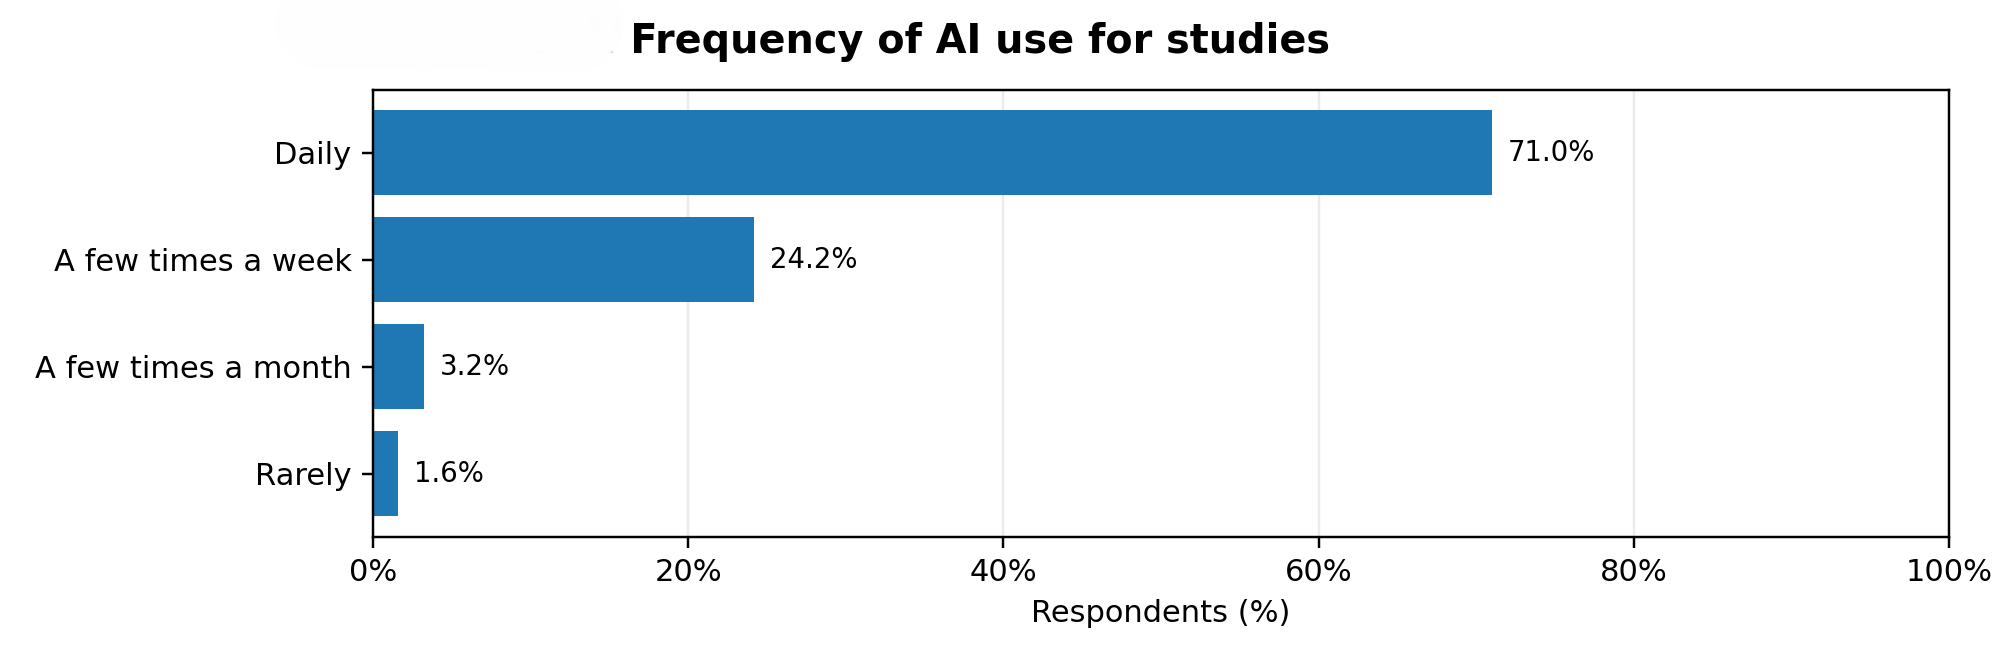
\includegraphics[width=0.88\linewidth]{charts/figure_5_1_ai_usage_frequency.png}
    \caption{Frequency of AI use for studies}
    \label{fig:ai-frequency}
\end{figure}

As shown in Figure~\ref{fig:ai-tools}, ChatGPT was the most frequently selected tool, reported by 90.3\% of respondents. Claude was selected by 67.7\%, while Google Gemini was selected by 54.8\%. Since respondents could select more than one tool, these percentages are not expected to total 100\%. The pattern suggests that students commonly use multiple AI platforms rather than relying on a single tool.

\begin{figure}[htbp]
    \centering
    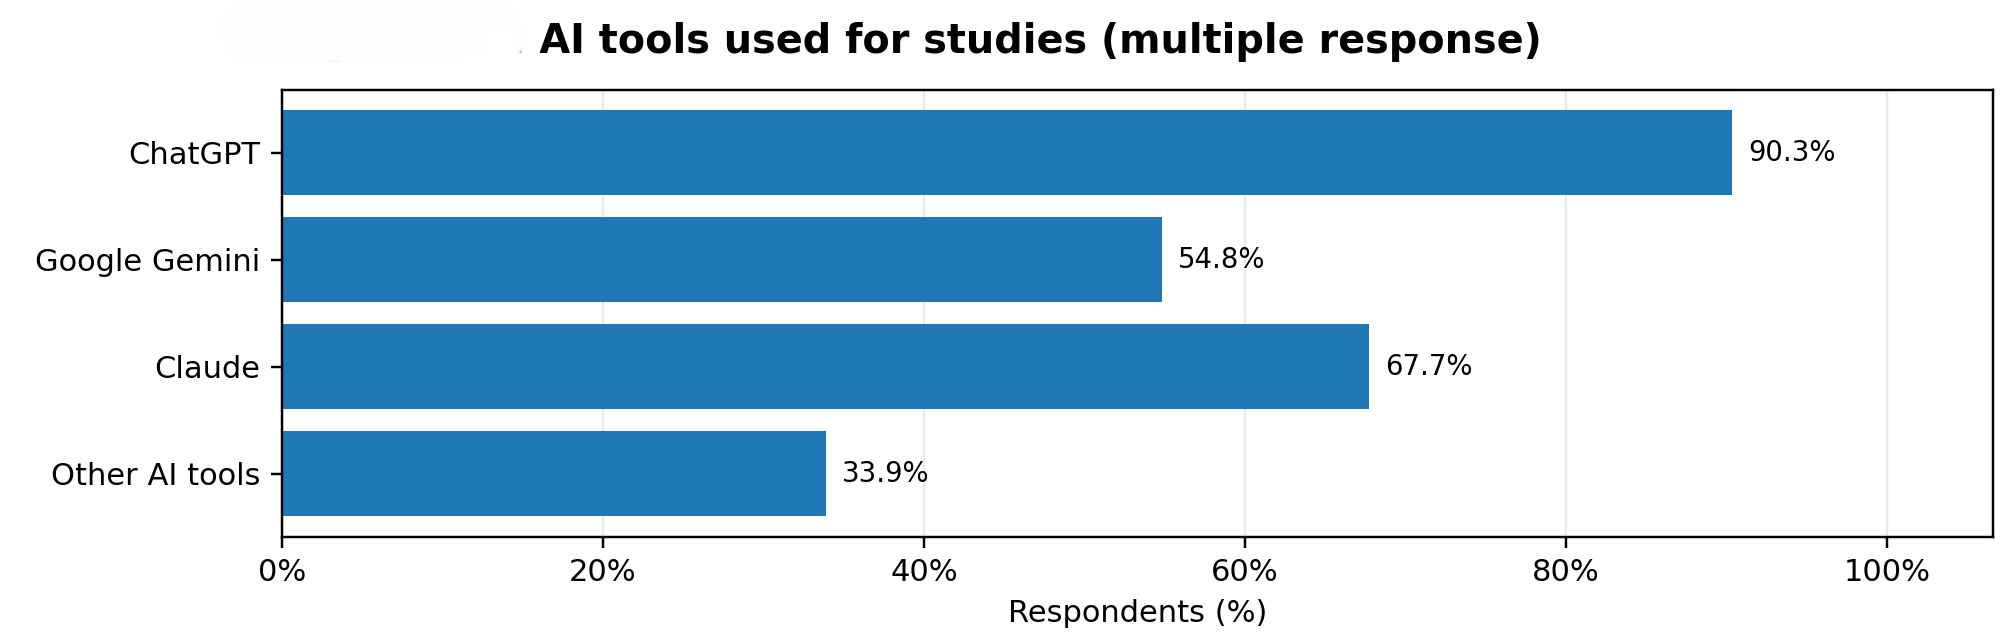
\includegraphics[width=0.88\linewidth]{charts/figure_5_2_ai_tools.png}
    \caption{AI tools used for academic purposes (multiple responses permitted)}
    \label{fig:ai-tools}
\end{figure}

Figure~\ref{fig:ai-purposes} summarizes the main academic purposes for which students reported using AI. Understanding difficult concepts was the most common purpose, selected by 91.9\% of respondents. Preparing notes and summaries was selected by 75.8\%, while 69.4\% selected examination preparation and 64.5\% selected programming or mathematical problem-solving. AI use therefore extends beyond obtaining direct answers and includes explanation, revision, and support for academic tasks.

\begin{figure}[htbp]
    \centering
    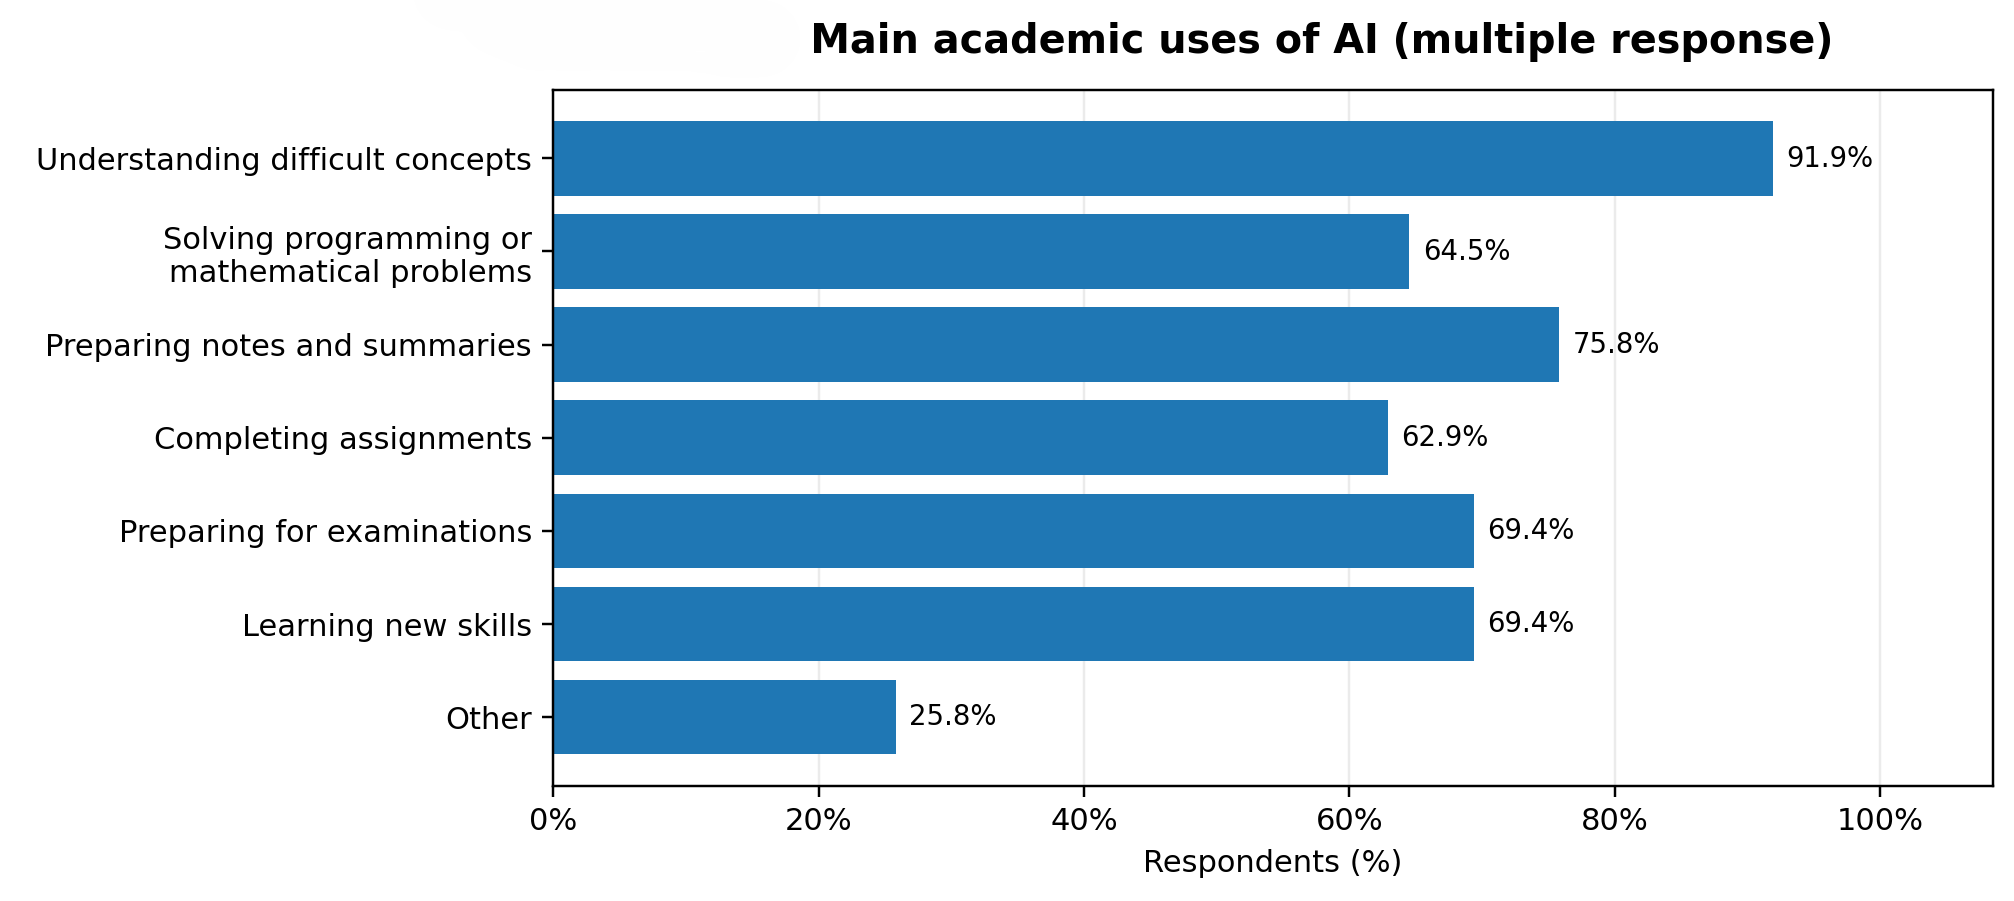
\includegraphics[width=0.88\linewidth]{charts/figure_5_3_ai_purposes.png}
    \caption{Main academic uses of AI (multiple responses permitted)}
    \label{fig:ai-purposes}
\end{figure}

Figure~\ref{fig:ai-timing} illustrates when students turn to AI. The most frequently selected situations were seeking help after getting stuck (73.8\%) and checking whether an answer was correct (70.5\%). Because respondents could select more than one situation, these results describe overlapping habits. They suggest that AI is used both as a source of assistance during difficulty and as a tool for checking work.

\begin{figure}[htbp]
    \centering
    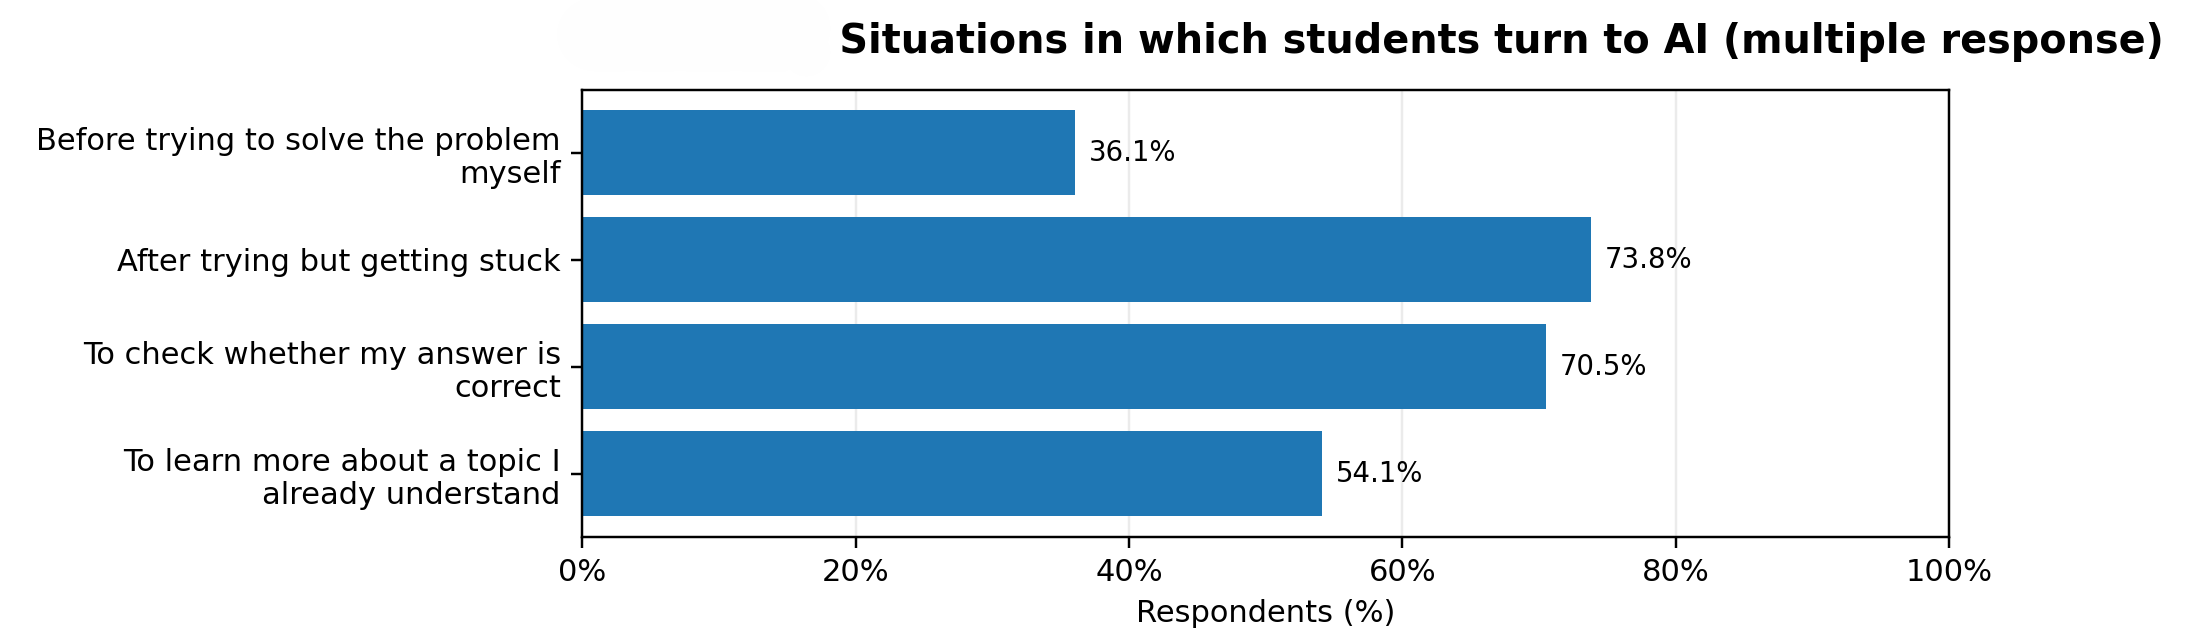
\includegraphics[width=0.88\linewidth]{charts/figure_5_4_when_ai_used.png}
    \caption{Situations in which students turn to AI (multiple responses permitted)}
    \label{fig:ai-timing}
\end{figure}

\subsection{Perceived Advantages of AI in Education}
\label{subsec:ai-advantages}

Figure~\ref{fig:time-saved} presents students' perceptions of time saved while studying. Approximately 60.7\% reported that AI saves them a lot of time, while 37.7\% reported that it saves them some time. Only a very small proportion selected very little time saved. These responses indicate that most respondents perceive AI as a time-saving study aid.

\begin{figure}[htbp]
    \centering
    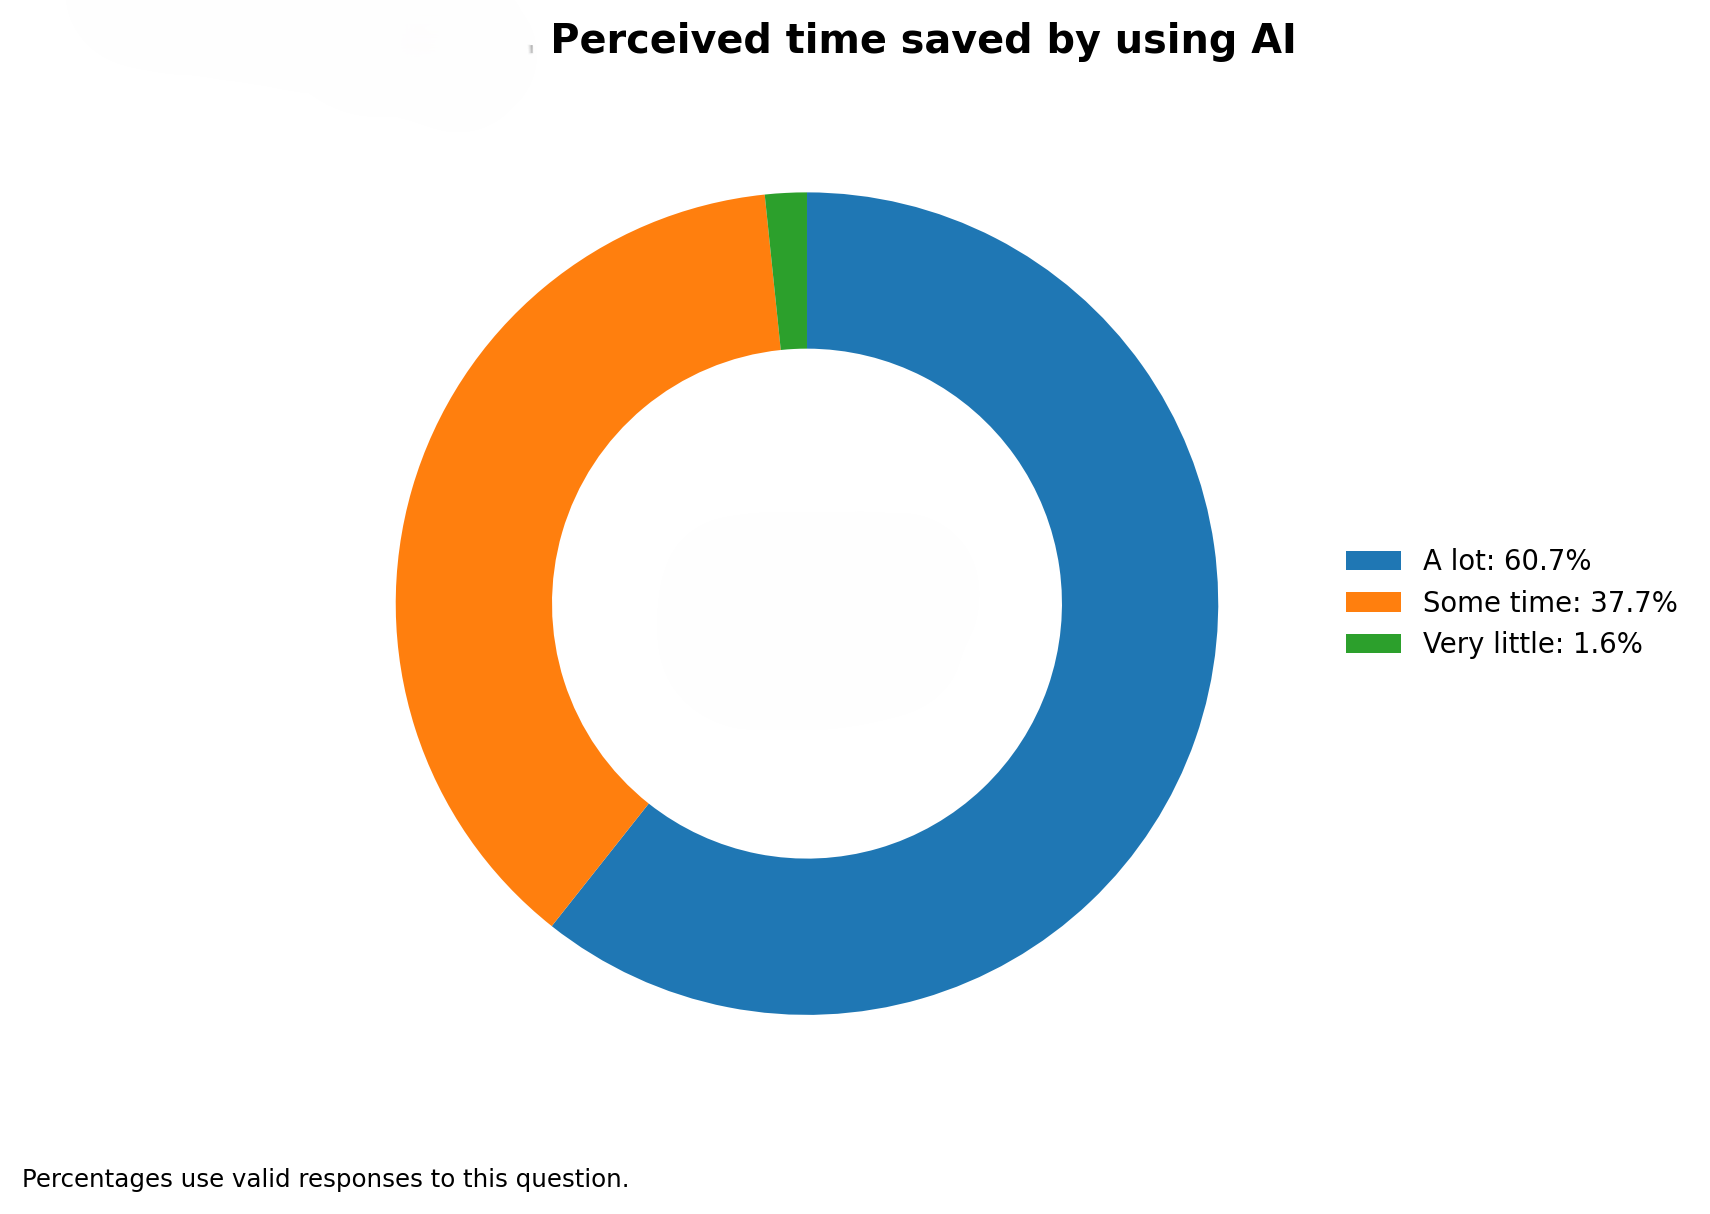
\includegraphics[width=0.82\linewidth]{charts/figure_5_5_time_saved_donut.png}
    \caption{Perceived time saved by using AI}
    \label{fig:time-saved}
\end{figure}

Figure~\ref{fig:learning-benefits} groups responses concerning understanding, explanation, and learning previously difficult material. A combined 80.3\% reported that AI always or often helps them understand difficult topics. In addition, 96.7\% said AI had helped them learn something they previously found difficult at least a few times. Responses comparing AI explanations with textbooks or classroom teaching were more varied, suggesting that the perceived usefulness of AI explanations may depend on the learner or topic.
As presented in Figure~\ref{fig:exam-convenience}, 91.8\% responded that AI helps with examination preparation either yes or to some extent. Furthermore, 86.9\% agreed or strongly agreed that AI makes learning more convenient by providing help when needed. Overall, the responses indicate positive perceptions of AI as an accessible study resource. These findings represent students' opinions and do not independently establish improvements in examination results.

\begin{figure}[htbp]
    \centering
    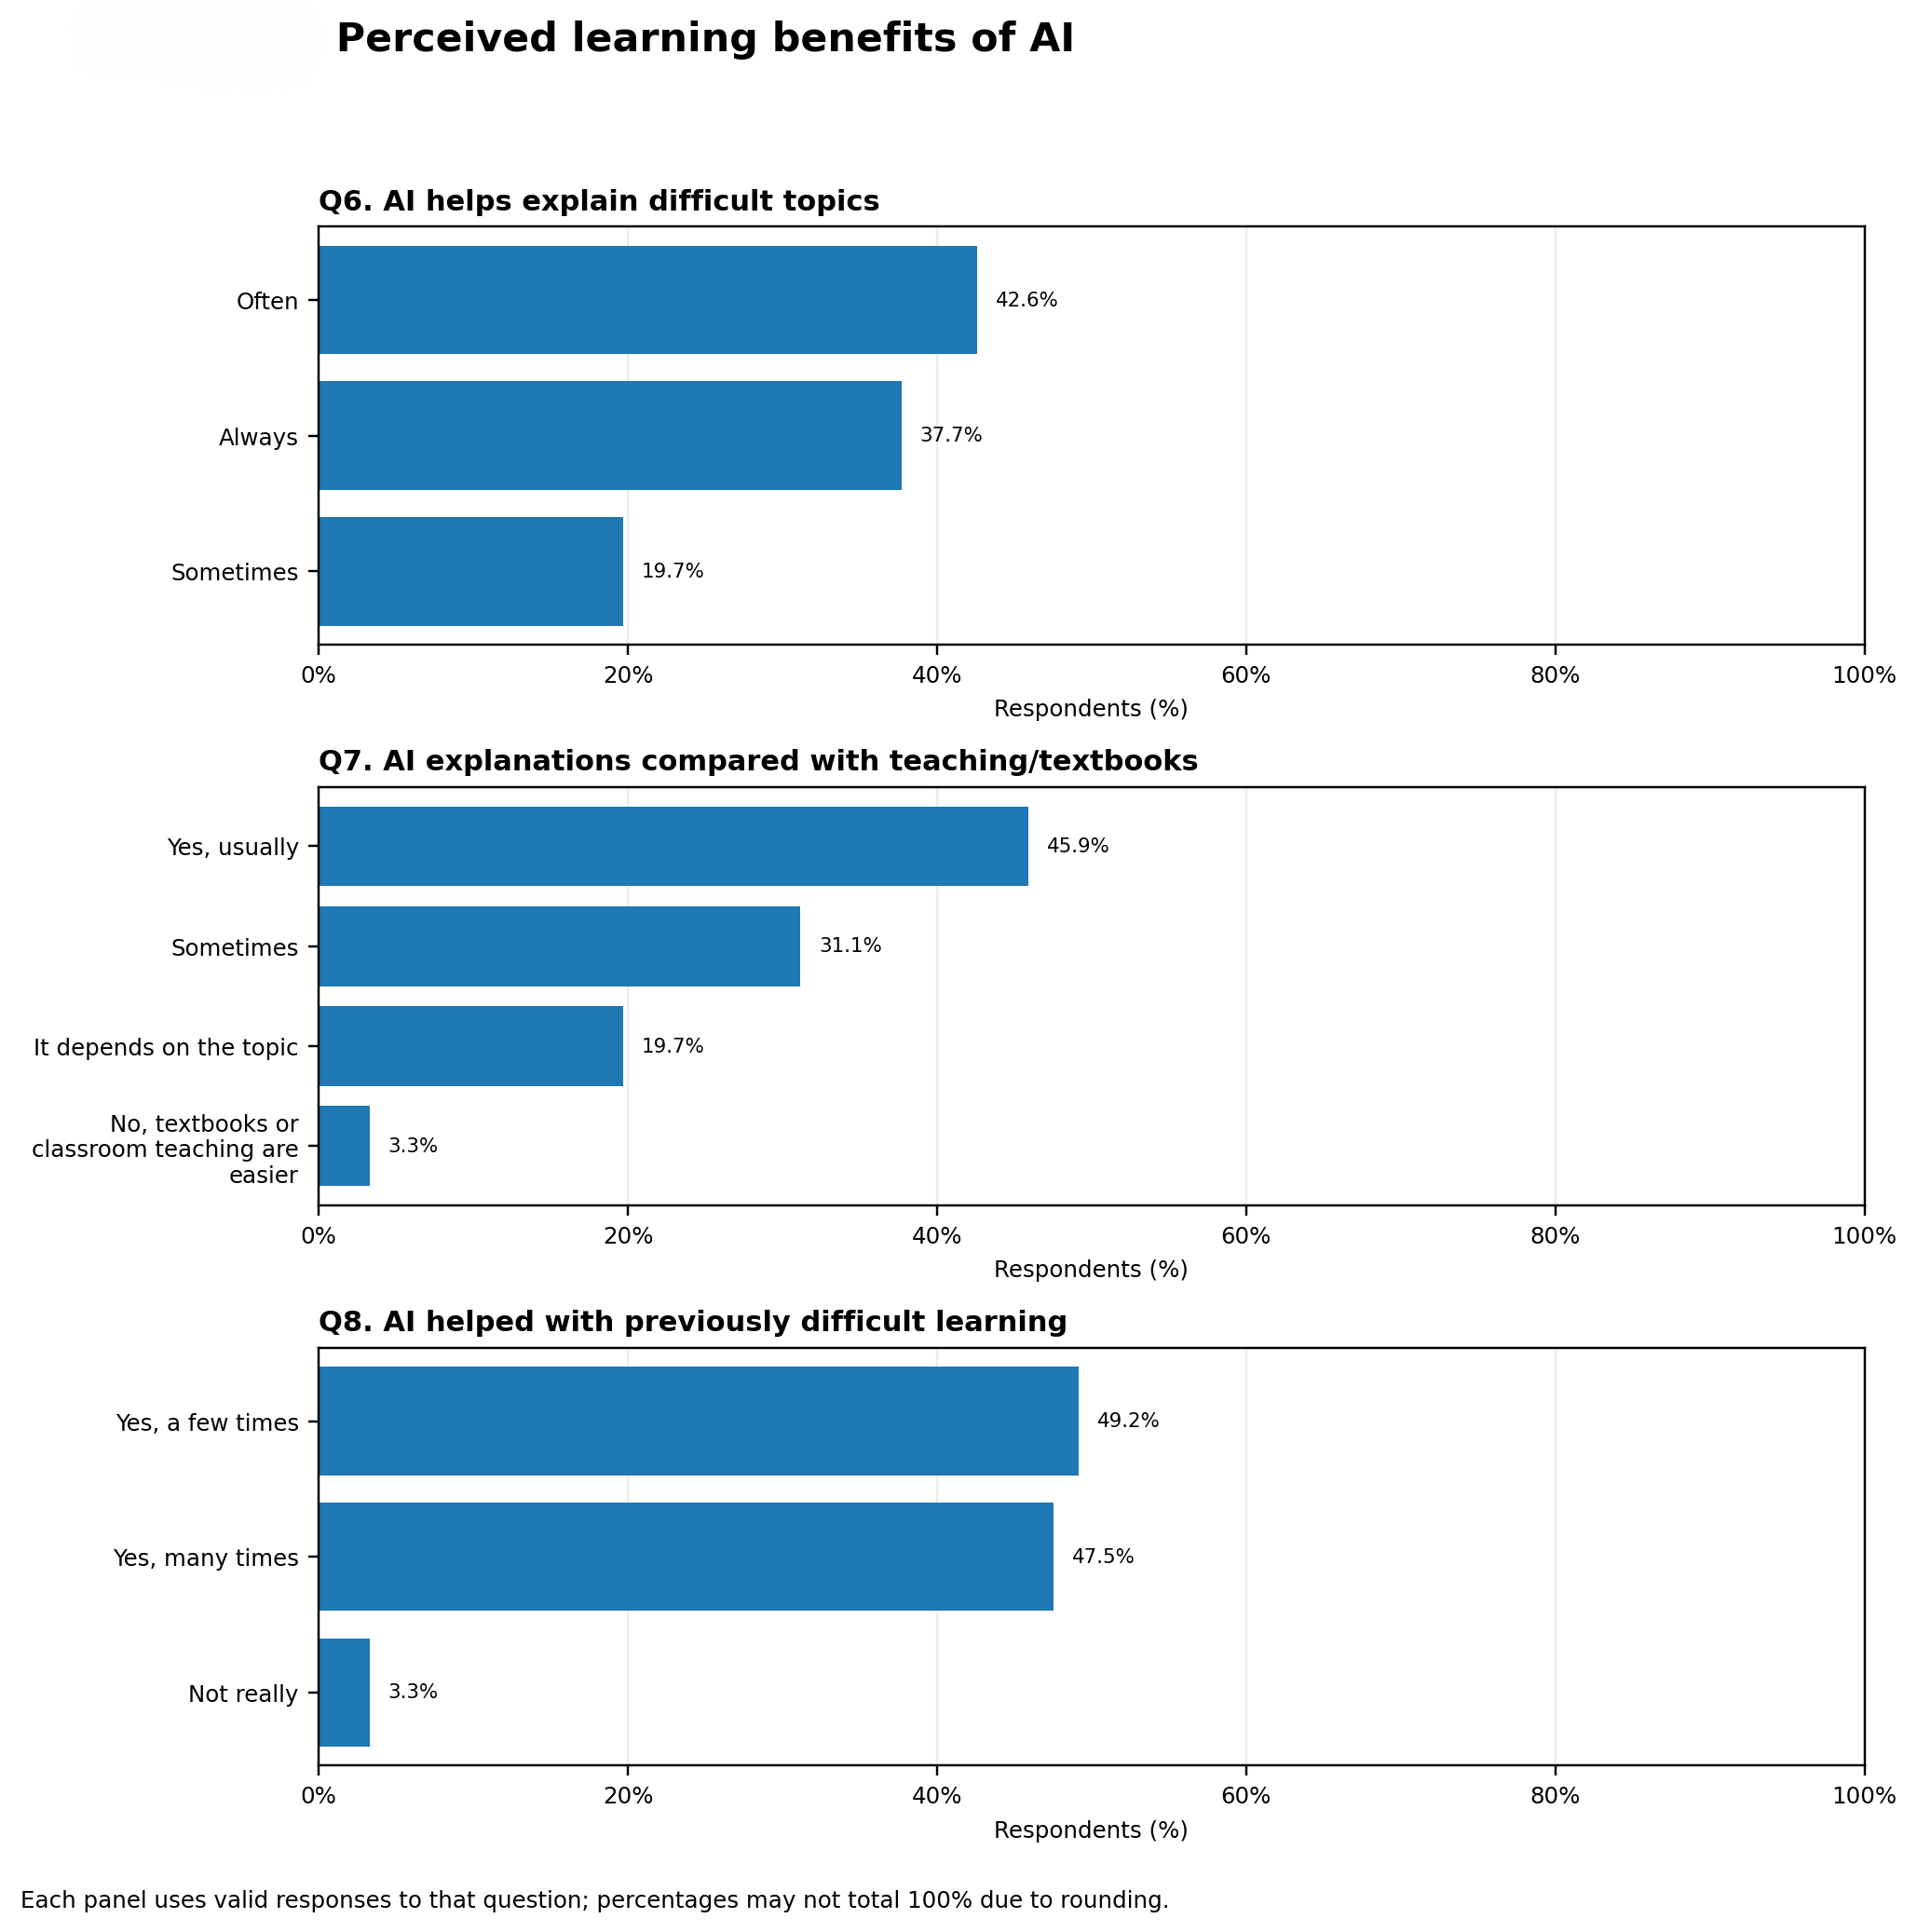
\includegraphics[width=0.88\linewidth]{charts/figure_5_6_learning_benefits.png}
    \caption{Perceived learning benefits of AI}
    \label{fig:learning-benefits}
\end{figure}

\begin{figure}[htbp]
    \centering
    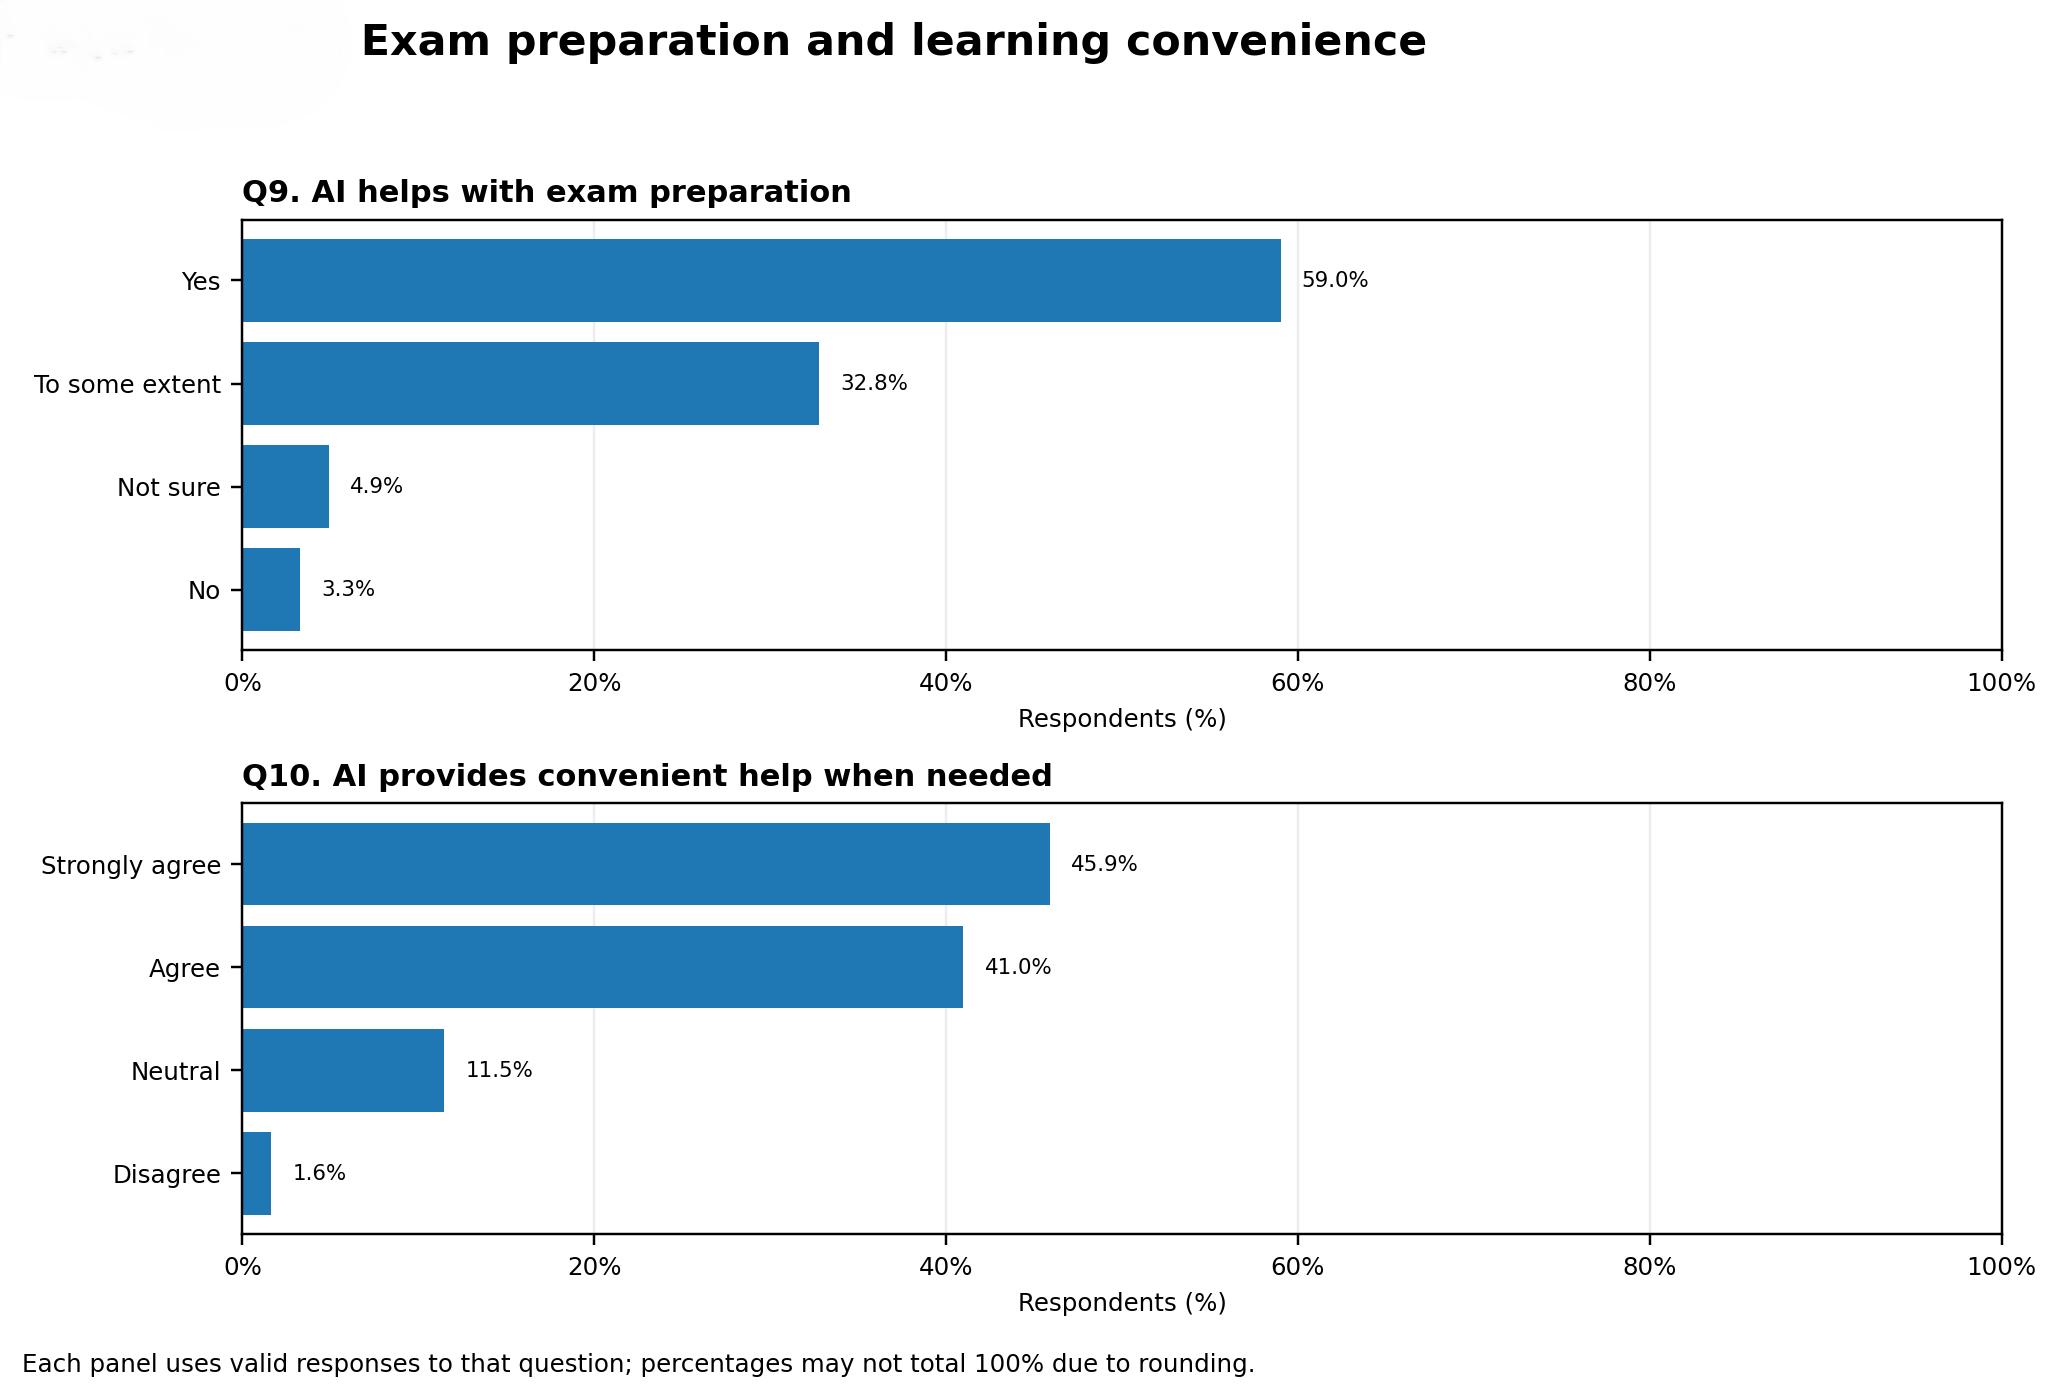
\includegraphics[width=0.88\linewidth]{charts/figure_5_7_exam_convenience.png}
    \caption{Perceived support for examination preparation and learning convenience}
    \label{fig:exam-convenience}
\end{figure}

\subsection{Perceived Disadvantages and Risks of AI}
\label{subsec:ai-disadvantages}

\begin{figure}[htbp]
    \centering
    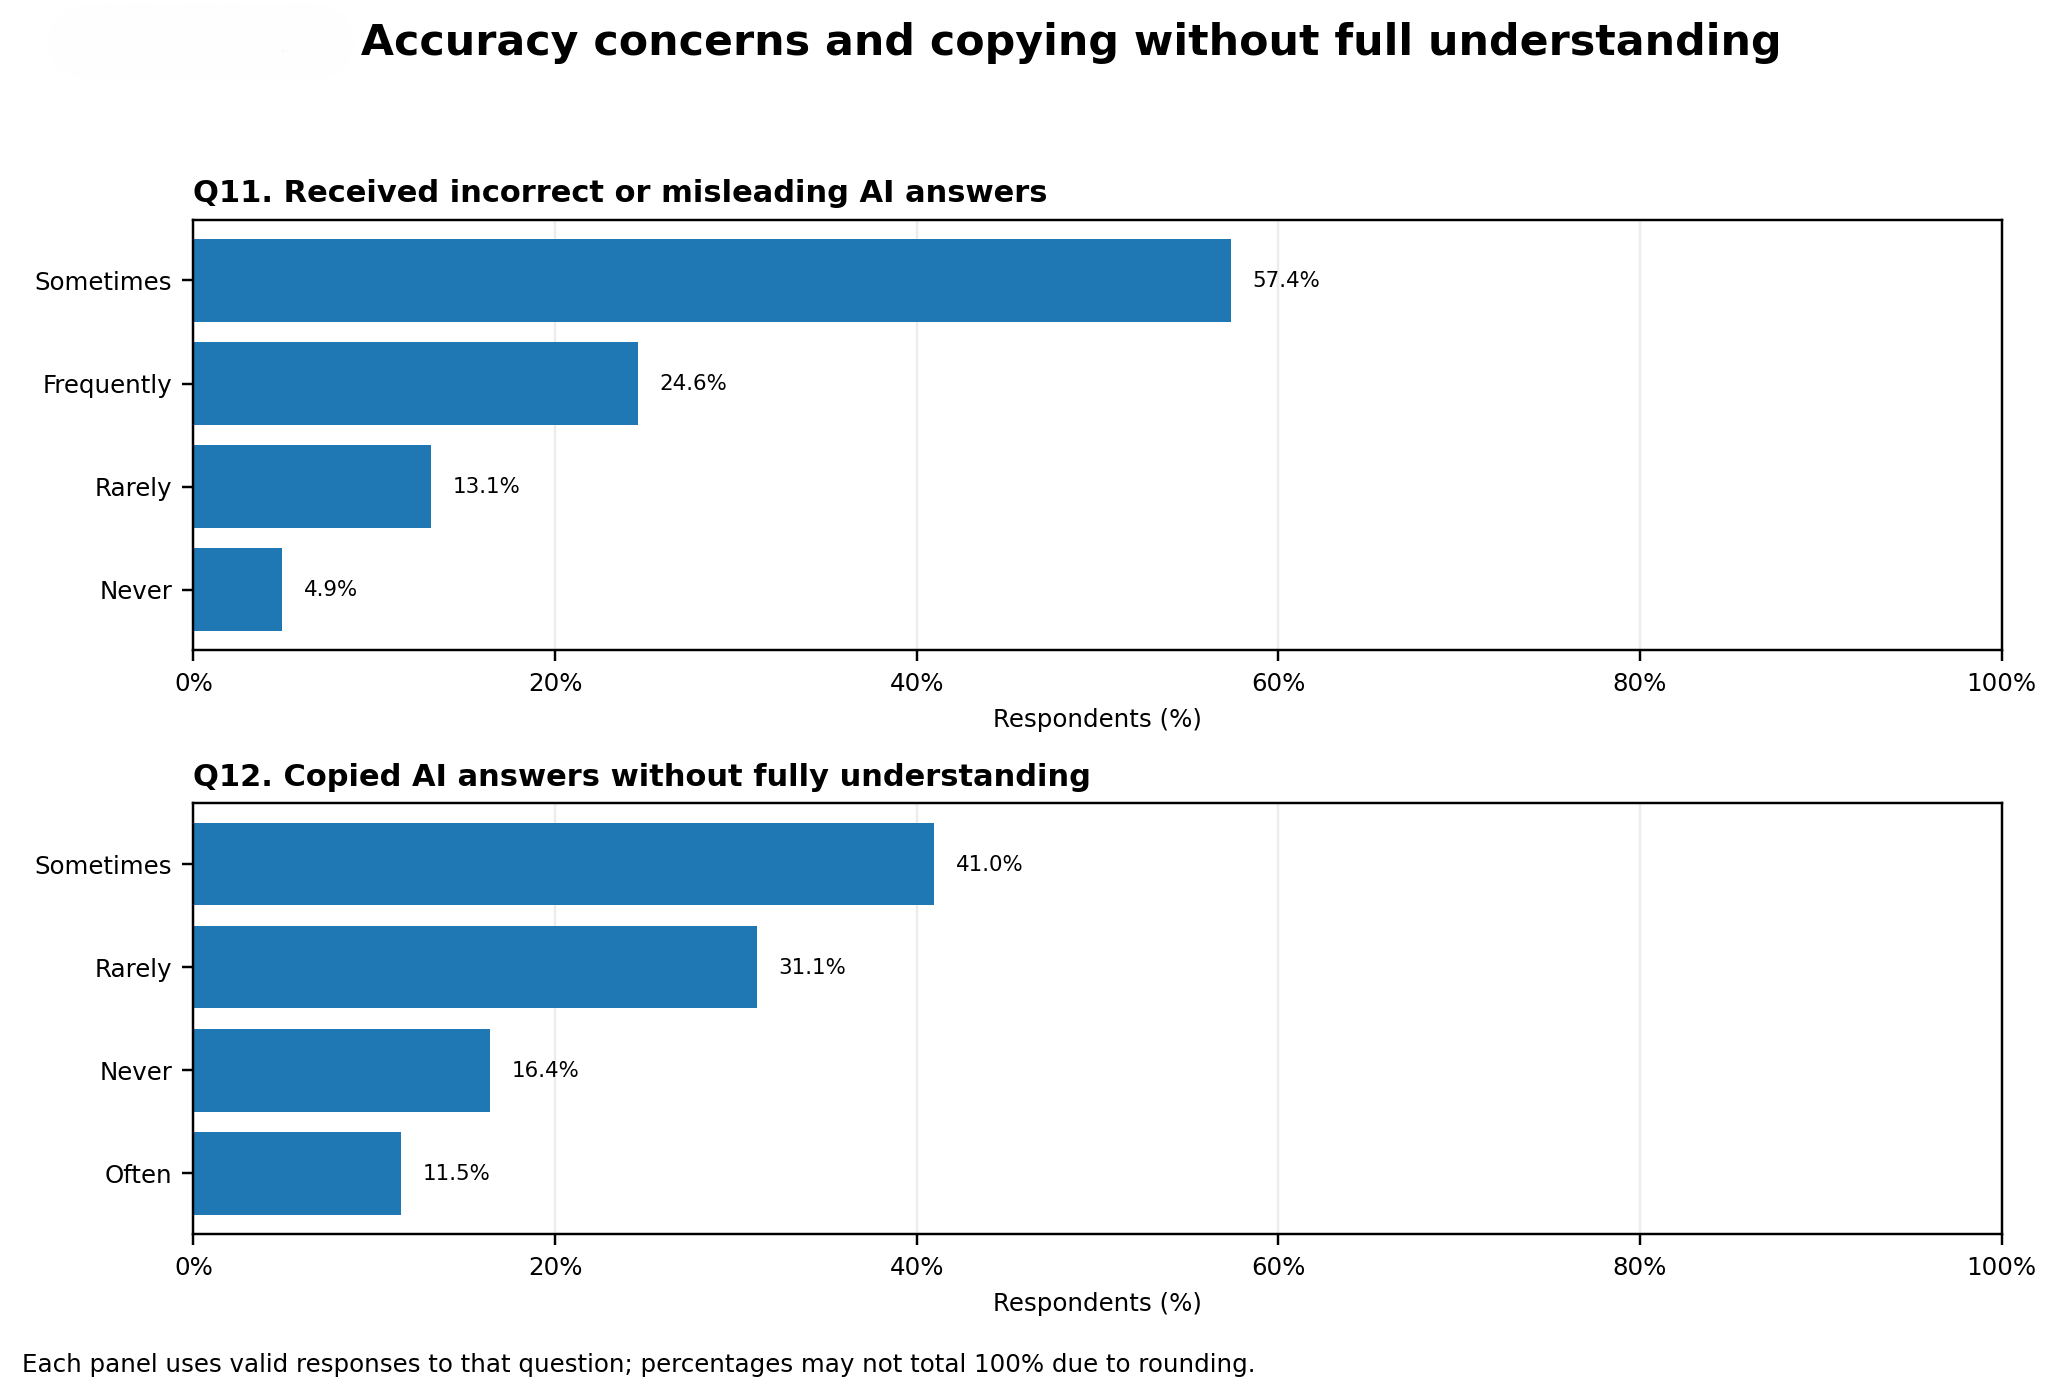
\includegraphics[width=0.88\linewidth]{charts/figure_5_8_accuracy_copying.png}
    \caption{Experiences with inaccurate answers and copying without full understanding}
    \label{fig:accuracy-copying}
\end{figure}


Figure~\ref{fig:accuracy-copying} presents responses about incorrect AI answers and copying without full understanding. A combined 82.0\% reported receiving an incorrect or misleading AI answer frequently or sometimes. In addition, 52.5\% reported that they often or sometimes copied an AI-generated answer without fully understanding it. These results highlight two concerns: AI-generated content may require verification, and using an answer without understanding it may limit the learning gained from the task.


\subsection{AI and Independent Learning}
\label{subsec:independent-learning}

Figure~\ref{fig:independent-learning} brings together perceptions of independent problem-solving, motivation, and verification practices. A combined 78.7\% agreed or strongly agreed that excessive AI use can reduce students' independent problem-solving skills. Separately, 75.0\% reported that they sometimes or often feel less motivated to solve problems independently when AI is available. These findings reflect perceived risks and self-reported habits; they do not prove that AI use directly causes a reduction in independent learning.

\begin{figure}[htbp]
    \centering
    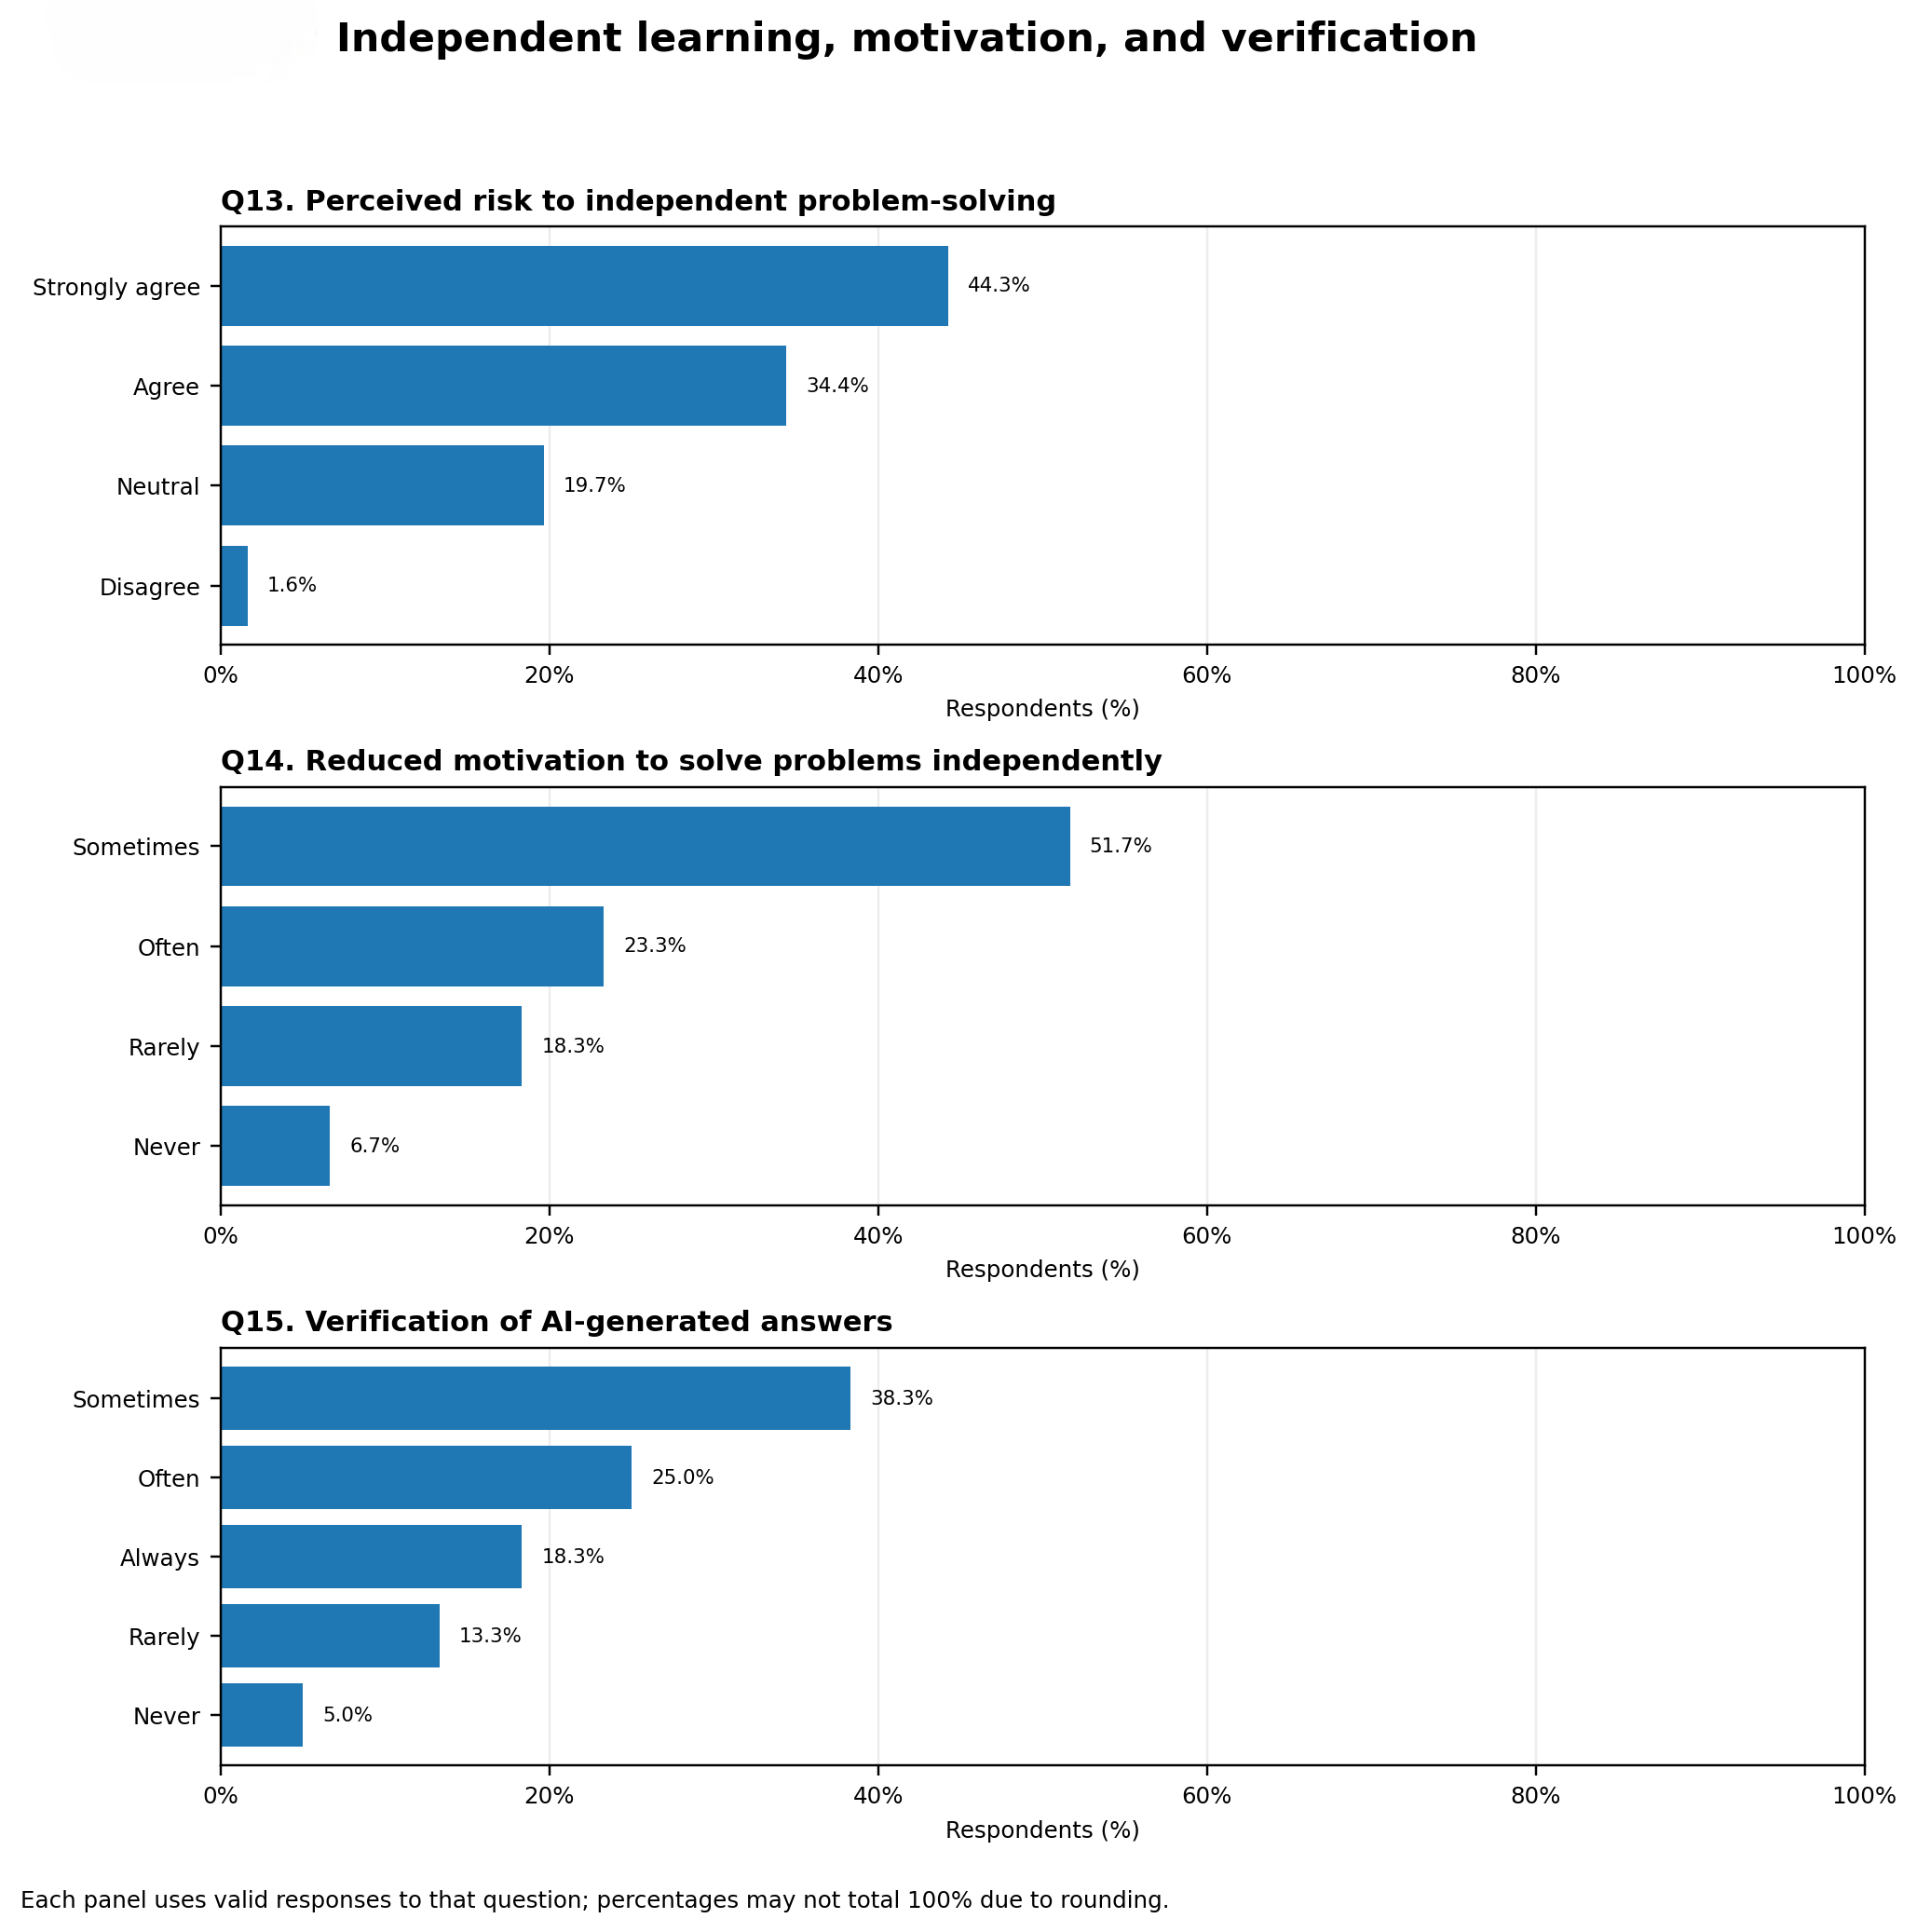
\includegraphics[width=0.88\linewidth]{charts/figure_5_9_independent_learning.png}
    \caption{Independent problem-solving, motivation, and verification practices}
    \label{fig:independent-learning}
\end{figure}

Verification practices are also important. Only 43.3\% reported always or often checking AI-generated answers using textbooks, teachers, or other reliable sources. This suggests an opportunity to encourage students to check important claims and use AI explanations alongside established learning resources.

Figure~\ref{fig:independent-confidence} shows students' confidence in completing academic work if AI tools were unavailable. Around 59.0\% described themselves as very or somewhat confident, while others selected neutral or lower confidence levels. This distribution suggests that confidence in working without AI varies across respondents. The result should be interpreted alongside their reported use habits and verification practices rather than as a direct measure of actual independent ability.

\begin{figure}[htbp]
    \centering
    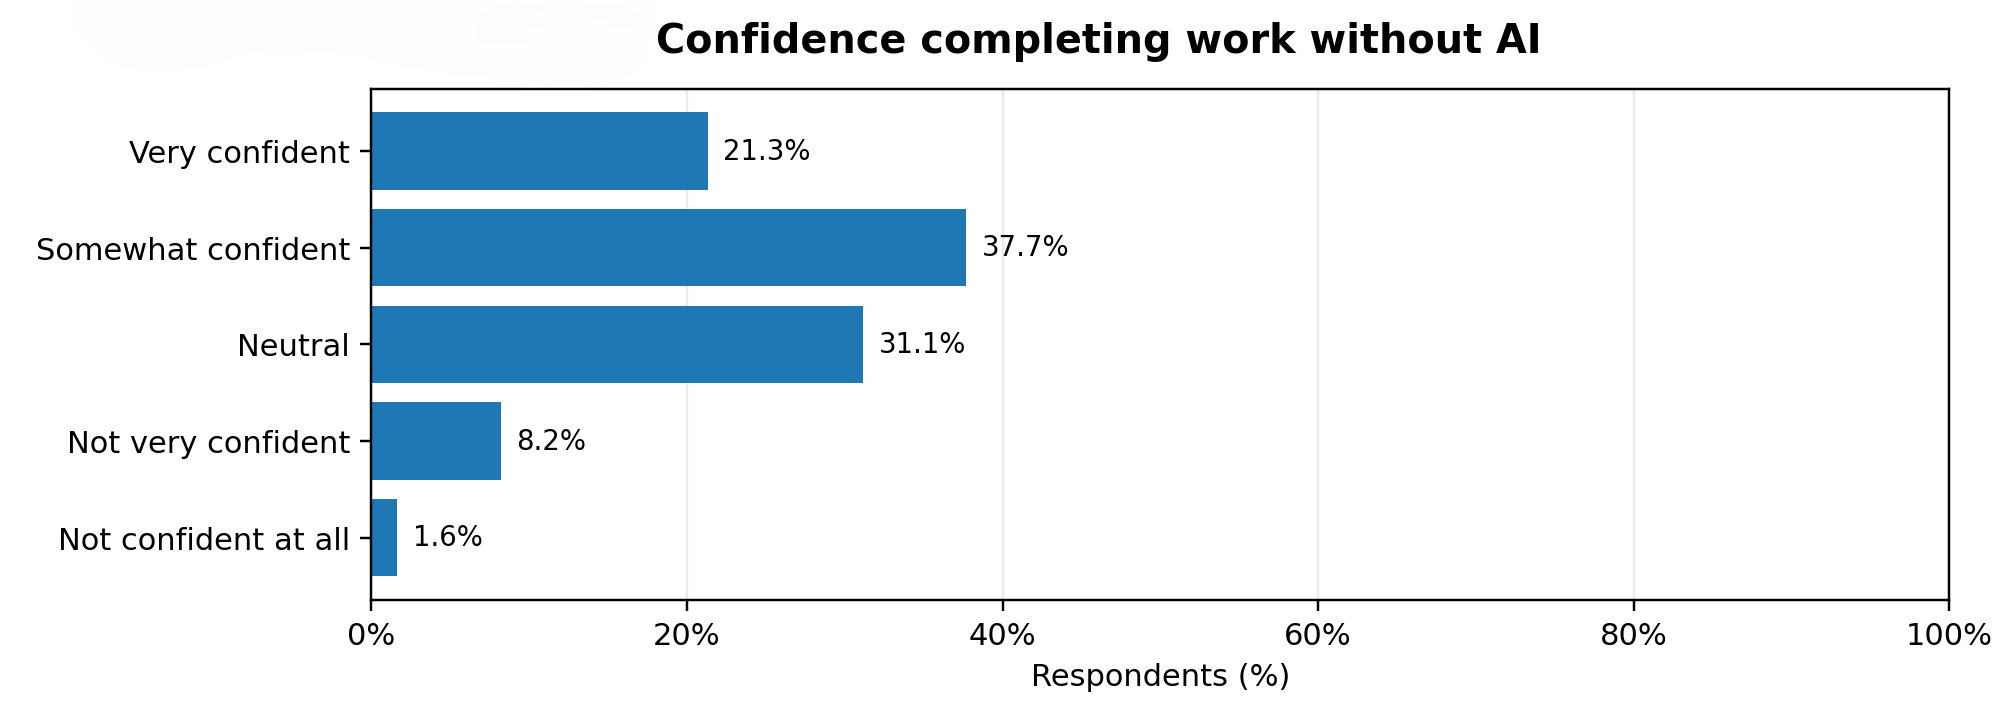
\includegraphics[width=0.88\linewidth]{charts/figure_5_12_independent_confidence.png}
    \caption{Confidence in completing academic work without AI}
    \label{fig:independent-confidence}
\end{figure}

\subsection{Perceived Impact on Academic Performance}
\label{subsec:academic-performance}
\begin{figure}[htbp]
    \centering
    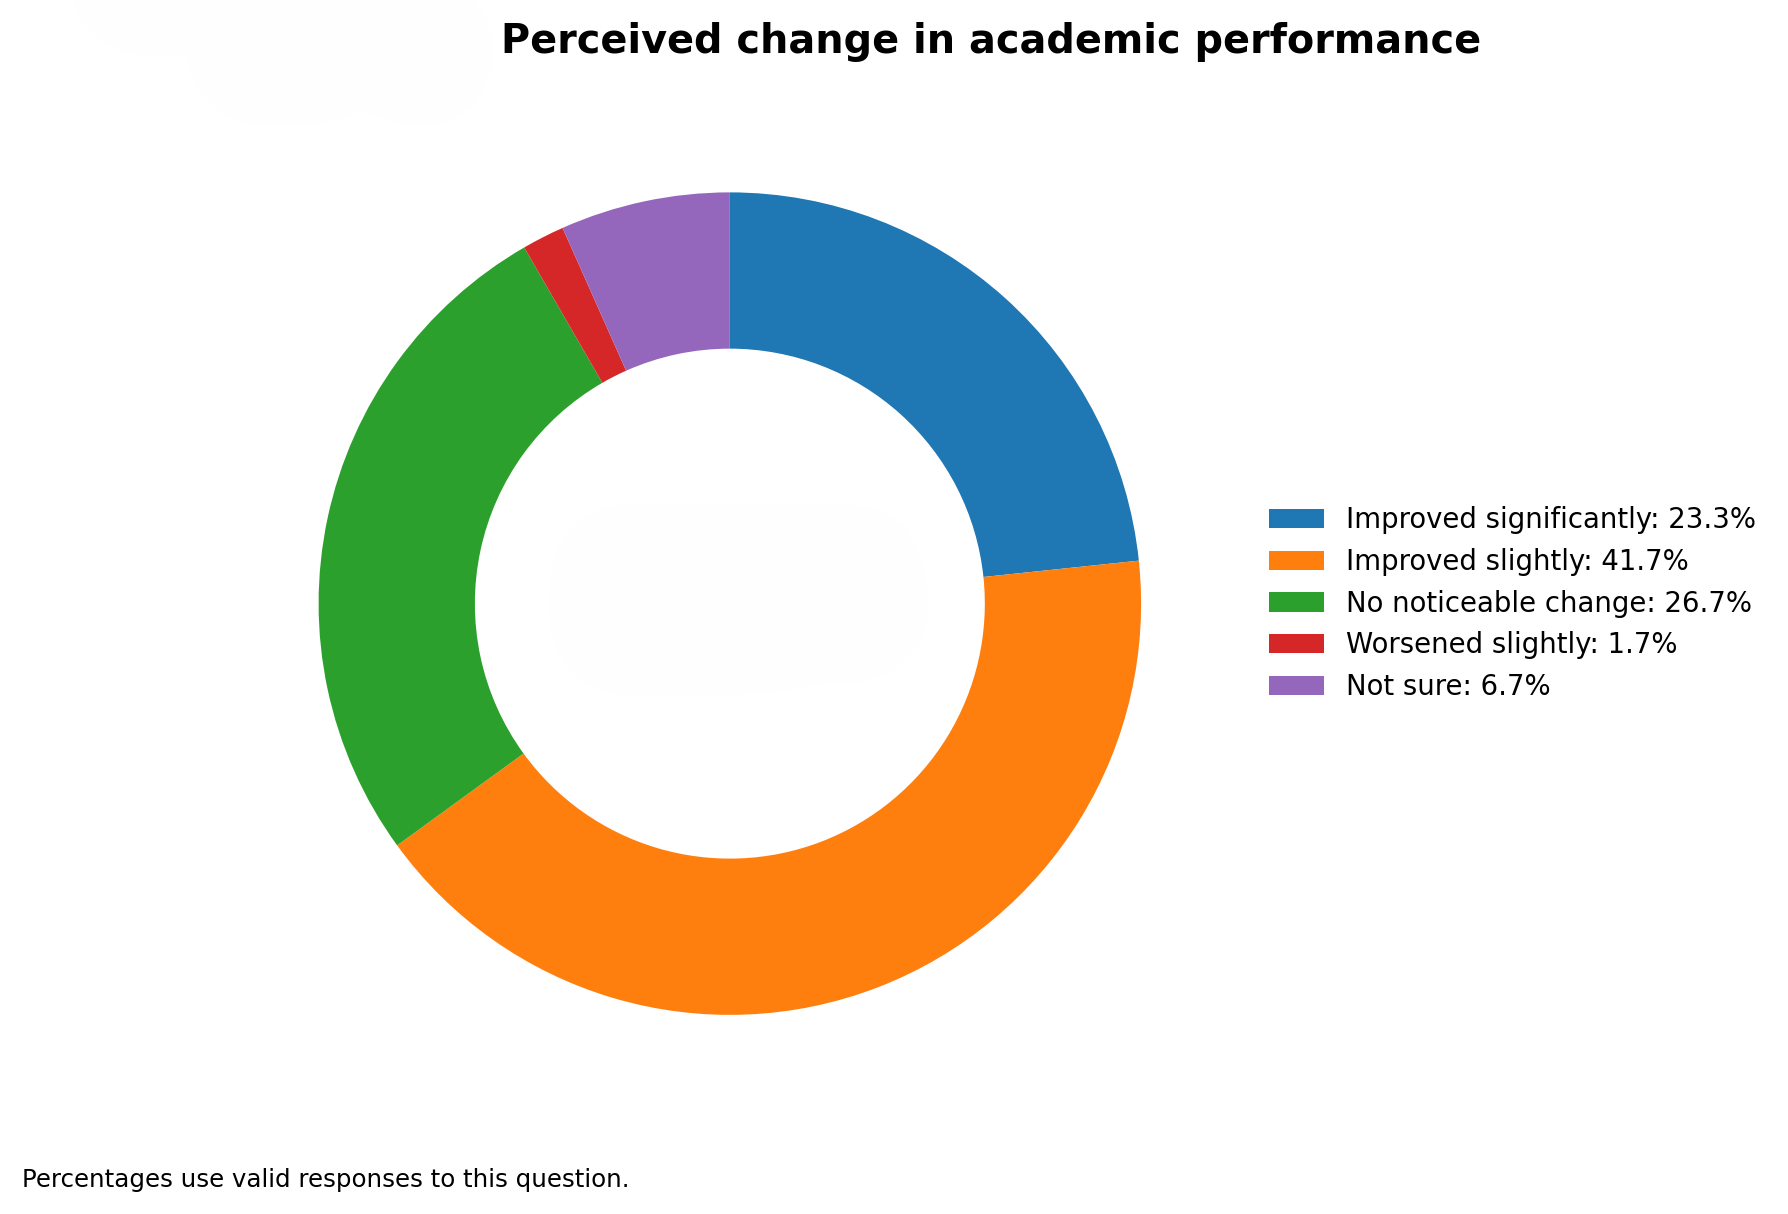
\includegraphics[width=0.82\linewidth]{charts/figure_5_10_performance_donut.png}
    \caption{Students' perceived change in academic performance}
    \label{fig:performance-change}
\end{figure}

Figure~\ref{fig:performance-change} summarizes students' reported changes in academic performance since they began using AI. Among the valid responses, 65.0\% reported that their performance had improved either slightly or significantly, while 26.7\% reported no noticeable change. A small proportion reported a slight decline, and some respondents were unsure. These are self-reported perceptions; grades were not independently measured, and the survey design cannot establish that AI caused any reported change.
\begin{figure}[htbp]
    \centering
    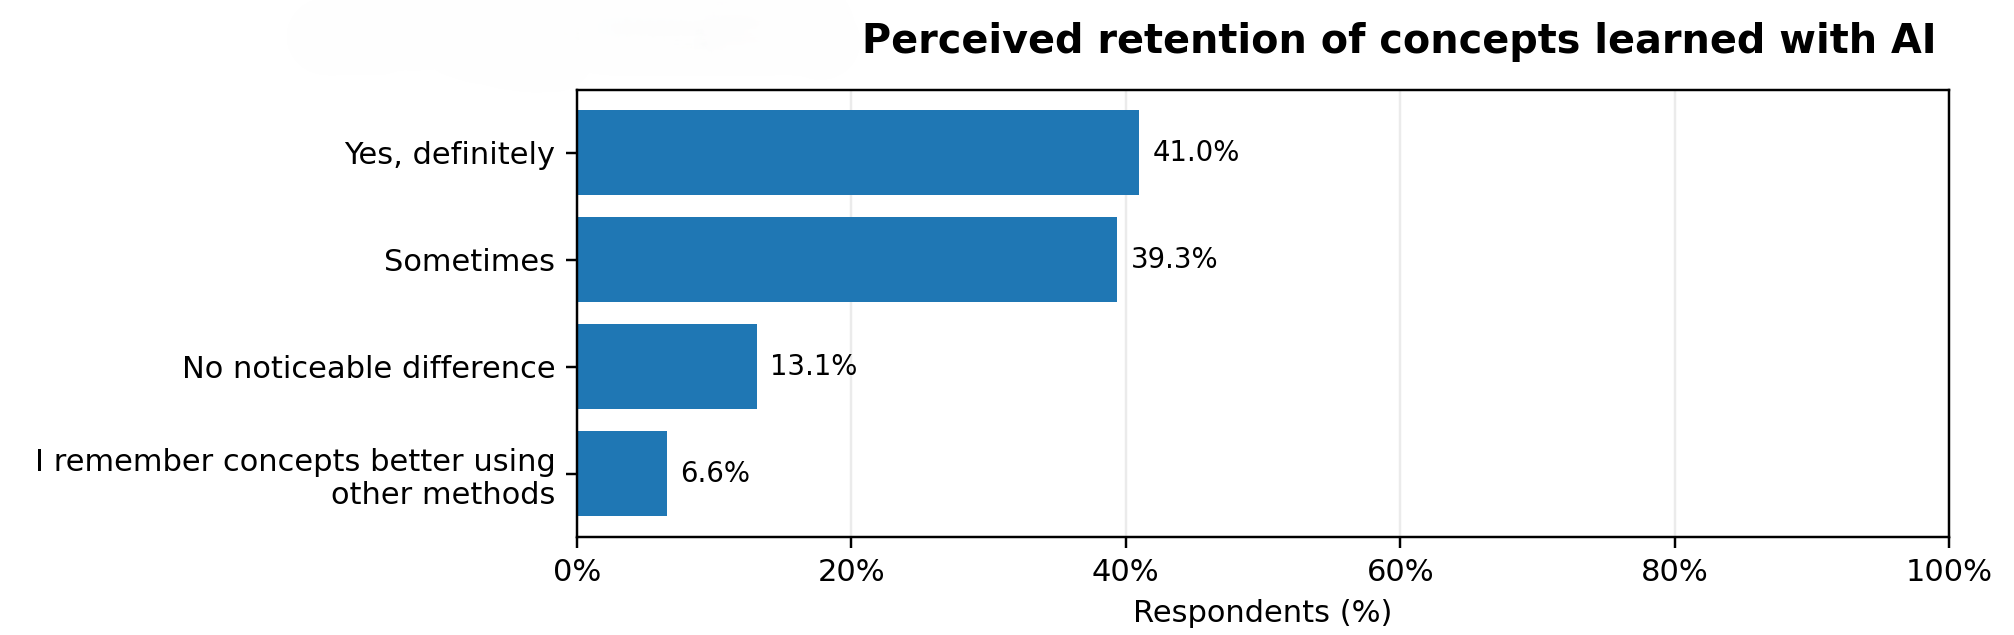
\includegraphics[width=0.88\linewidth]{charts/figure_5_11_concept_retention.png}
    \caption{Perceived retention of concepts learned with AI explanations}
    \label{fig:concept-retention}
\end{figure}
Figure~\ref{fig:concept-retention} concerns perceived retention of concepts learned with AI explanations. A combined 80.3\% selected either yes, definitely or sometimes when asked whether they remember concepts better with AI explanations. Other respondents reported no noticeable difference or better retention through alternative methods. The results indicate that many students perceive a learning benefit, although the survey does not objectively test memory or long-term retention.

\subsection{Overall Opinions on AI in Education}
\label{subsec:overall-opinion}

Figure~\ref{fig:overall-opinion} summarizes the overall view of AI and the preferred approach to its use in education. The most common response to the overall-impact question was that AI has both positive and negative effects, selected by 57.4\%. A further 36.1\% viewed its impact as very or somewhat positive. This indicates that respondents generally recognize benefits while also acknowledging potential drawbacks.

\begin{figure}[htbp]
    \centering
    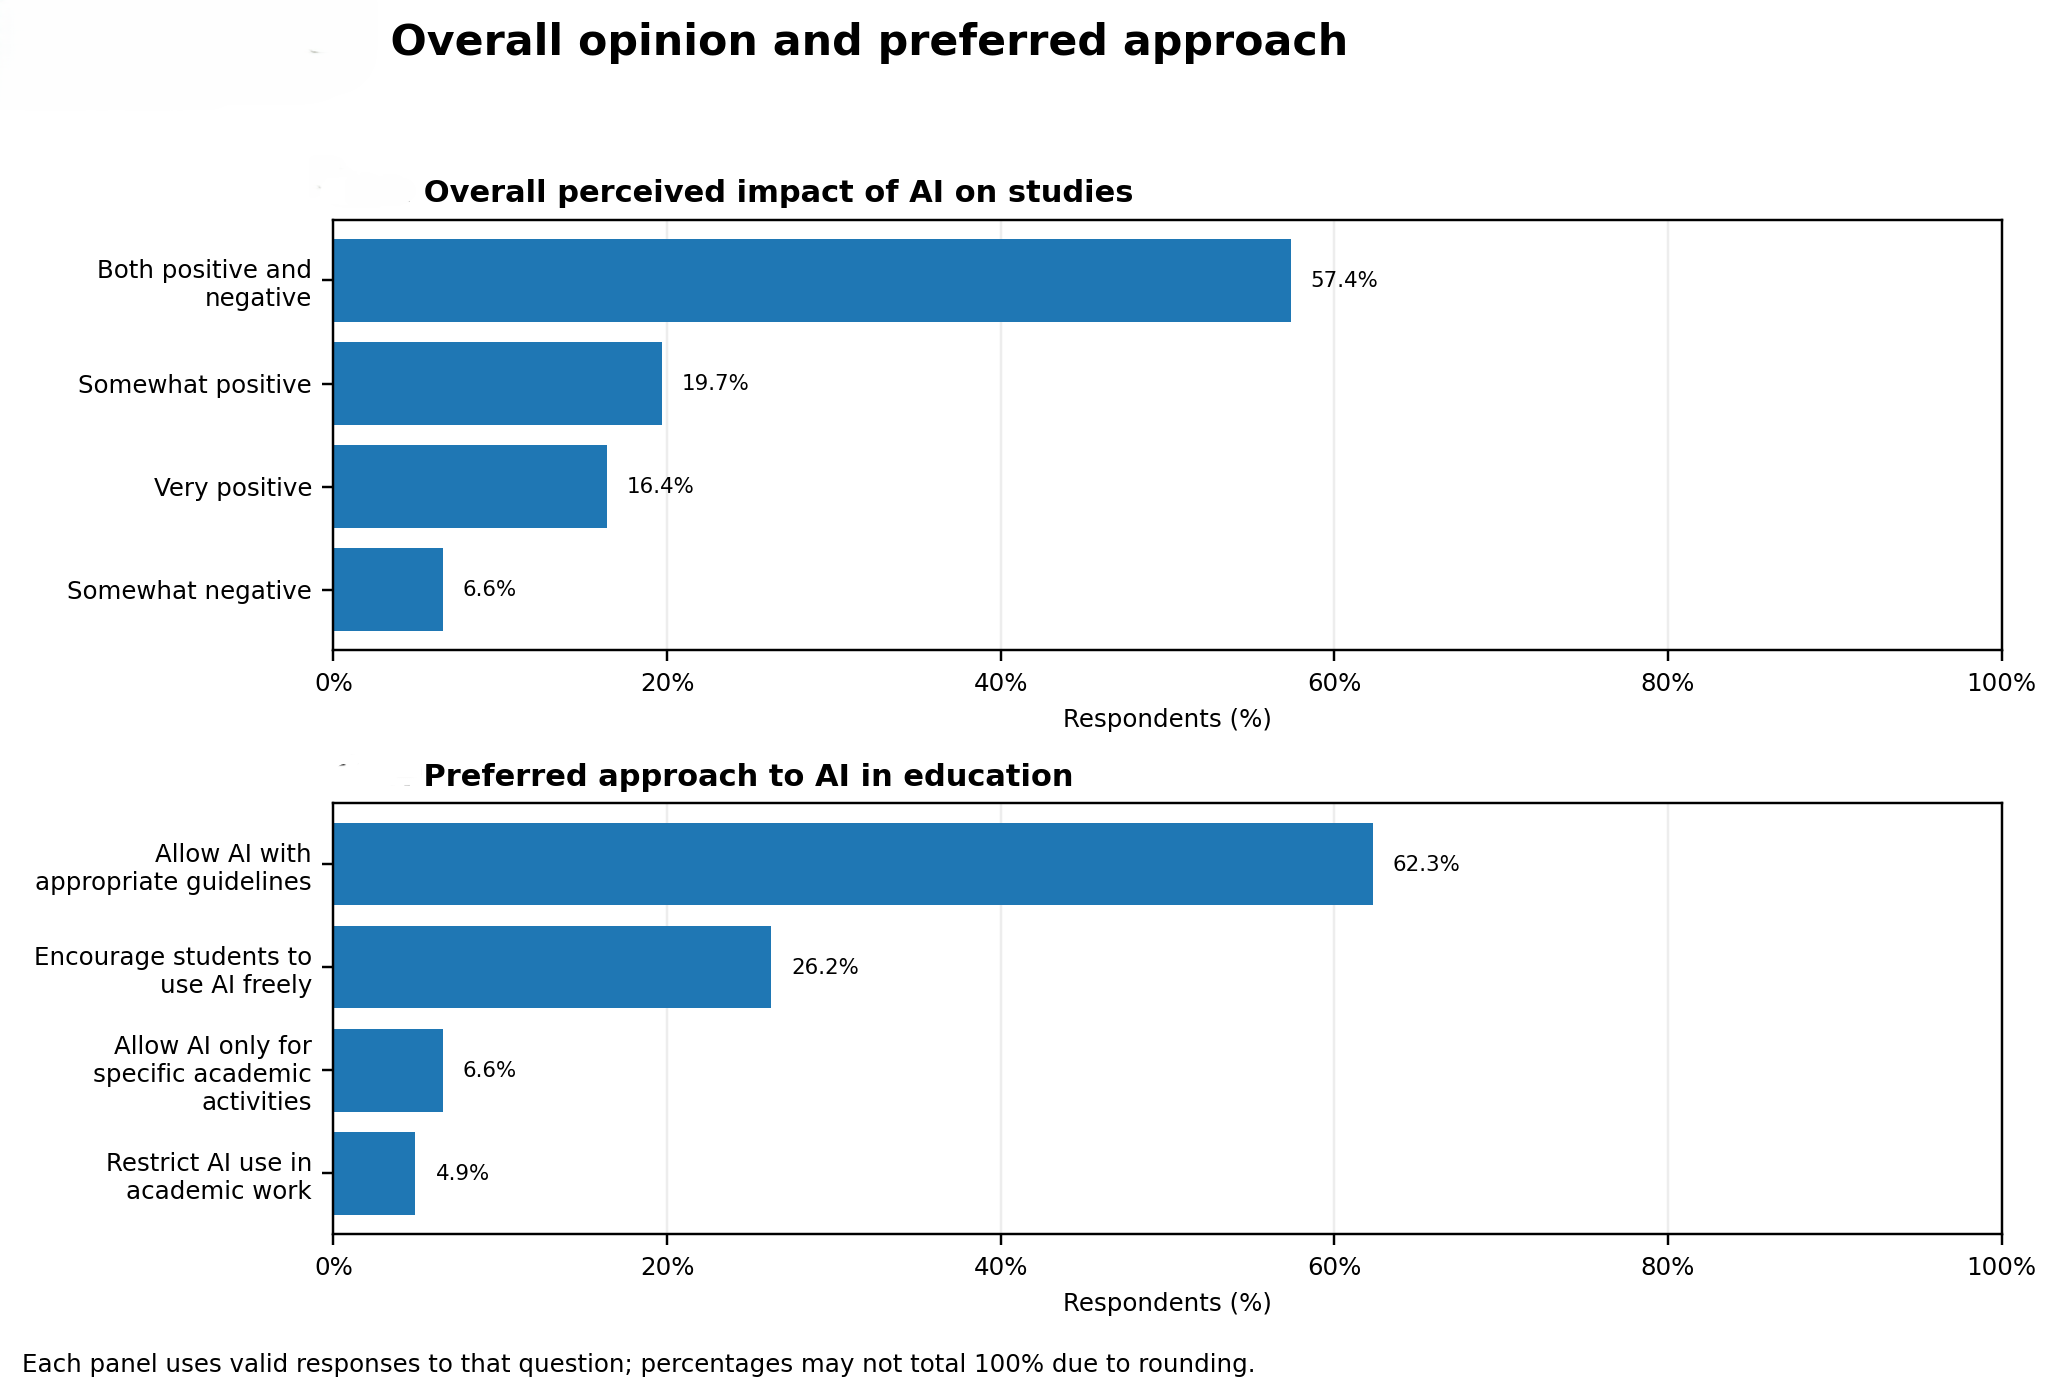
\includegraphics[width=0.88\linewidth]{charts/figure_5_13_overall_opinions.png}
    \caption{Overall perceived impact of AI and preferred approach to its use in education}
    \label{fig:overall-opinion}
\end{figure}

Regarding educational policy, 62.3\% preferred allowing AI with appropriate guidelines, while 26.2\% supported encouraging students to use AI freely. The preference for guidelines suggests that many respondents favor access to AI alongside expectations for responsible use, independent effort, and verification of generated information.

\subsection{Summary of Survey Results}
\label{subsec:survey-summary}

Overall, the survey responses show frequent use of AI for academic purposes and generally positive perceptions of its usefulness for understanding concepts, saving time, and preparing for examinations. At the same time, respondents reported encountering inaccurate answers, and many expressed concern about possible effects on independent problem-solving. Verification of AI-generated information was not consistently reported as a frequent practice. Most respondents favored allowing AI in education with appropriate guidelines rather than unrestricted use or a complete restriction.

These findings should be interpreted within the scope of this descriptive survey. The responses reflect students' experiences and opinions, not experimentally verified effects. The following sections discuss the advantages and disadvantages in greater detail and consider recommendations for responsible AI use in education.



\section{Advantages of AI in Education}
\label{sec:advantages-ai}

The survey responses indicate that students generally perceive Artificial Intelligence (AI) as a useful academic support tool. One of the clearest reported benefits is assistance with understanding difficult concepts. Most respondents indicated that AI had helped them learn something they previously found difficult, suggesting that students value the ability to request explanations, examples, and alternative ways of presenting information.

Another perceived advantage is the convenience of receiving help when it is needed. Respondents commonly reported that AI supports examination preparation and helps them save study time. AI tools can provide quick explanations, summarize lengthy material, generate practice questions, and assist students in reviewing topics at their own pace. Such functions may be particularly useful when students need additional practice outside classroom hours.

The responses also show that students use AI for several academic purposes, including preparing notes and summaries, solving programming or mathematical problems, completing assignments, and learning new skills. This variety suggests that students view AI not only as a question-answering tool but also as a flexible resource for different stages of learning.

However, the benefits depend on how AI is used. When students ask follow-up questions, compare explanations, solve practice problems, and verify information, AI can support active learning. Its usefulness should therefore be understood as assistance that complements students' own effort, rather than as a replacement for textbooks, teachers, or independent thinking.

\section{Disadvantages of AI in Education}
\label{sec:disadvantages-ai}

Although the survey indicates several perceived benefits, respondents also identified risks associated with using AI for academic work. A notable concern is the possibility of receiving incorrect or misleading information. AI-generated responses can sound convincing even when they contain factual errors, incomplete explanations, or outdated details. Students should therefore avoid treating every generated answer as authoritative.

The responses also indicate that some students sometimes copy AI-generated answers without fully understanding them. This practice may help complete a task quickly, but it can reduce opportunities to practise reasoning, problem-solving, and explaining concepts independently. If students rely on ready-made answers without examining the reasoning behind them, their immediate task completion may not translate into deeper learning.

Another concern is the perceived effect of frequent AI use on independent problem-solving. Many respondents expressed agreement with the view that excessive use could weaken independent skills, and a substantial proportion reported sometimes or often feeling less motivated to solve problems themselves when AI is available. These results describe students' perceptions and reported habits; they do not demonstrate that AI use directly causes a decline in ability.

The survey also points to the importance of verification. Not all respondents reported checking AI-generated information consistently against textbooks, teachers, or other reliable sources. Limited verification can allow mistakes to go unnoticed and may lead students to use unreliable information in assignments or examination preparation.

Finally, students may become overly dependent on AI if they use it before making an independent attempt. For this reason, AI use should be balanced with unaided practice, reading, discussion, and reflection. The central issue is not simply whether students use AI, but whether they use it critically and responsibly.

\section{Findings and Discussion}
\label{sec:findings-discussion}

The survey findings reveal several patterns in students' use and perception of AI in education.

\begin{enumerate}
    \item \textbf{AI is a regular part of study routines.}
    The responses show that AI use is frequent among the surveyed students, with daily use representing the largest frequency category. ChatGPT was the most commonly selected tool in the dataset, while other AI tools were also used by a substantial proportion of respondents. This indicates that students are engaging with a range of AI platforms for academic support.

    \item \textbf{Conceptual understanding is a major reason for using AI.}
    Understanding difficult concepts was the most frequently selected academic purpose. Students also reported using AI to prepare notes, revise for examinations, solve programming or mathematical problems, and complete assignments. This suggests that AI is integrated into several types of academic activity.

    \item \textbf{Students generally perceive AI as helpful.}
    A large proportion of respondents reported that AI had helped them learn difficult material, supported examination preparation, and made learning more convenient. Many also perceived AI as saving study time. These findings point to the perceived value of accessible explanations and on-demand academic assistance.

    \item \textbf{Accuracy and over-reliance remain concerns.}
    Many respondents reported encountering incorrect or misleading AI answers. More than half reported sometimes or often copying an answer without fully understanding it. These patterns highlight the need to verify AI-generated content and to focus on understanding rather than simply obtaining a completed answer.

    \item \textbf{Students recognize potential risks to independent learning.}
    Respondents expressed concern that excessive AI use could affect independent problem-solving, and many reported sometimes or often feeling less motivated to solve problems on their own. At the same time, the responses to the question about confidence without AI were mixed. This suggests that students' confidence in independent academic work varies across the surveyed group.

    \item \textbf{Perceived academic improvement should be interpreted cautiously.}
    Many respondents reported that their academic performance had improved since they began using AI, and many felt that AI explanations helped them remember concepts. However, the study relies on self-reported perceptions and does not compare verified grades or measure learning outcomes experimentally. The results therefore cannot establish that AI caused an improvement in academic performance.

    \item \textbf{Students favor guided use of AI.}
    The most common overall opinion was that AI has both positive and negative effects. The most frequently selected policy preference was to allow AI with appropriate guidelines. This indicates support for a balanced approach that recognizes educational benefits while addressing accuracy, academic integrity, and independent learning.
\end{enumerate}

Taken together, the findings suggest that students see AI as a useful learning aid but also recognize risks related to inaccurate information and dependence. The results support an approach that emphasizes responsible use, verification, and active engagement with the material. As the study uses convenience sampling and self-reported responses, these conclusions apply primarily to the surveyed group and should not be generalized to all students without further research.

\section{Suggestions and Recommendations}
\label{sec:recommendations}

Based on the survey findings, the following recommendations may help students and educational institutions make more effective use of AI.

\begin{enumerate}
    \item \textbf{Use AI as a learning assistant, not a substitute for learning.}
    Students should attempt a question independently before requesting AI assistance. When AI provides a solution, students should review the steps and make sure they can explain the reasoning in their own words.

    \item \textbf{Verify important information.}
    AI-generated answers should be checked against textbooks, lecture materials, academic publications, teachers, or other reliable sources, especially when the information is used in assignments or examination preparation.

    \item \textbf{Encourage explanation-based prompts.}
    Rather than asking AI only for a final answer, students can request step-by-step explanations, simpler examples, practice questions, hints, or feedback on their own attempts. This can encourage understanding and active participation.

    \item \textbf{Maintain independent problem-solving practice.}
    Students should regularly complete exercises without AI assistance. Independent practice helps them assess what they know, identify gaps in understanding, and prepare for examinations or situations where AI tools are unavailable.

    \item \textbf{Establish clear academic guidelines.}
    Educational institutions should communicate when AI use is permitted, when it must be acknowledged, and which forms of AI-generated work are unacceptable. Guidelines should encourage transparency and responsible use rather than leaving expectations unclear.

    \item \textbf{Develop AI literacy.}
    Students should be taught that AI tools can produce incorrect, biased, incomplete, or fabricated information. Learning how to evaluate generated responses is an important part of using these tools effectively.

    \item \textbf{Use AI to support teachers rather than replace them.}
    AI may provide additional practice and personalized explanations, while teachers remain important for subject expertise, feedback, mentoring, and evaluating student understanding. A blended approach can combine the accessibility of AI with human guidance.

\end{enumerate}

These recommendations aim to preserve the perceived advantages of AI while reducing the risks identified in the survey. Their effectiveness would need to be evaluated in practice rather than assumed from the present descriptive study alone.

\section{Conclusion}
\label{sec:conclusion}

This case study examined students' reported use of Artificial Intelligence in education, including their usage habits, perceived benefits, concerns, and views on its overall impact. The survey indicates that AI tools are commonly used for understanding difficult concepts, preparing notes, solving academic problems, and preparing for examinations. Many respondents perceived AI as convenient and helpful for learning and time management.

At the same time, the responses reveal important concerns. Students reported encountering incorrect or misleading AI-generated answers, and some acknowledged copying answers without fully understanding them. Respondents also expressed concern about possible effects on independent problem-solving and indicated that verification practices could be more consistent. These findings demonstrate the importance of critical evaluation and responsible use.

Overall, the survey suggests that AI is best treated as a supplementary educational resource rather than a replacement for independent effort, teachers, or established learning materials. Appropriate guidance, verification of information, transparent academic rules, and regular independent practice may help students benefit from AI while reducing the risks of over-reliance.

The findings must be interpreted in light of the study's limitations. The survey relies on self-reported experiences and convenience sampling, and it does not establish a causal relationship between AI use and academic performance. Further research using broader samples and objective measures of learning outcomes would help clarify how AI affects student learning over time.

In conclusion, the educational value of AI depends not only on the availability of the technology but also on the way students and institutions use it. A balanced approach that combines AI assistance with independent thinking, verification, and responsible academic practice offers a practical direction for its use in education.

\begin{thebibliography}{9}

\bibitem{ucw}
University Canada West.
\newblock \emph{Advantages and Disadvantages of AI in Education}.
\newblock Available at: \url{https://www.ucanwest.ca/blog/education-careers-tips/advantages-and-disadvantages-of-ai-in-education}.
\newblock Accessed October 26, 2026.

\bibitem{klimova}
B. Klimova and M. Pikhart.
\newblock ``Exploring the effects of artificial intelligence on student and academic well-being in higher education: a mini-review.''
\newblock \emph{Frontiers in Psychology}, vol. 16, article 1498132, 2025.
\newblock \url{https://doi.org/10.3389/fpsyg.2025.1498132}.
\newblock Full text: \url{https://pmc.ncbi.nlm.nih.gov/articles/PMC11830699/}.

\bibitem{ijsret}
B. Prasad, Preeti, and Shireen-e-Sadaf.
\newblock \emph{Case Studies of AI in Education: Transforming Learning Experiences}.
\newblock IJSRET, December 3, 2025.
\newblock Available at: \url{https://ijsret.com/2025/12/03/case-studies-of-ai-in-education-transforming-learning-experiences/}.

\end{thebibliography}

\end{document}